\chapter{Parametric Modeling Results}

\section{Introduciton}
In this chapter I will present the results of parametric modeling in forecasting next year decarbonization rates. The chapter presents a sequence of models in increasing order of complexity that allow us to:
\begin{enumerate}
    \item Test key hypothesis on the relationship between the predictors and next year decarbonization rates. In particular, I followed the CDP structure in testing multiple sets of predictors groped based on focus areas, such as carbon credits, initiaties and incentives, risks and opportunites, to understand what role each area plays in next year decarbonization rate and which predictors are useful from each set. 
    \item Build a state-of-the-art model that strikes an optimal balance between number of features and prediction accuracy. To achieve this task, models were scored based on the Akaike information criterion (AIC), which is a method for selecting models that balance goodness of fit and model complexity, aiming to identify how new data might behave \cite{AIC}
\end{enumerate}
For each presented model, I will first present the key questions and hypothesis, then a brief model descriptions, the results, and a discussion. At each step, I will select the most relevant predictors and carry them to the next model. 

\subsection{Response Variable:}
\noindent Unless otherwise specified, most models are forecasting \textit{Next Year Decarbonization Rate} (distribution and further information are provided in the previous chapter corresponding to Figure \ref{fig:next-year-real-decarbonization-rate}), which is the year on year change in Real emissions for a given company espressed as a percentage. 

\section{Model I: Year and Current Decarbonization Rate}

\subsection{Key Hypothesis}
\begin{itemize}
    \item What is the relationship between previous year and next year decarbonization rate?
    \item What is the correlation between years and real decarbonization rate? In particular, is it the case that over time the rate of decarbonization is improving? 
    \item Do the unique characteristics of each firm matter in forecasting decarbonization? Will a mixed effect model using the unique firm identifier as a random effect be better than a simple OLS?
\end{itemize}

\subsection{Models} 
\begin{enumerate}
    \item Simple Ordinary Least Squares regression with intercept using Year and Same-Year Decarbonization Rate as predictors
    \item Linear Mixed Effect Model with the same predictors as model (1) but with an added random intercept for the unique firm identifier
\end{enumerate}
% Forecasting decarbonization rates is no easy task, especially because we are dealing with multiple time series, one for each firm, which have a realtively low number of data-points. The maximum length of a timeseries is $12$ years, which applies to only $370$ for firms which reported all years from $2011$ to $2022$. The average number of reporting years is $6$. A forecasting exercise can be very helpful for multiple reasons:
% \begin{itemize}
%     \item Understanidng the current capabilities when it comes to forecasting next year decarbonization rates. Setting up a benchmark in the field to understand to what extent CDP data can be used to determine future rates.
%     \item Identifying the most important predictors: in the analysis I tried intentionally as many predicots as possible to select the most relevant features. This task is very important as it can allow the CDP survey to iterate and improve the questions to capture details on the most relevant data points when it comes to tracking real decarbonization rates
%     \item Determine which decarbonization activities have an effect in the future: while it is true that 
% \end{itemize}

\begin{table}[H] \centering    \caption{Model Comparison: Fixed Effects Only vs. Random Intercept for Firm Id}    \label{tab:R1}  \small  \resizebox{0.8\textwidth}{!}{\begin{tabular}{@{\extracolsep{5pt}}lcc}  \\[-1.8ex]\hline  \hline \\[-1.8ex]   & \multicolumn{2}{c}{\textit{Dependent variable:}} \\  \cline{2-3}  \\[-1.8ex] & \multicolumn{2}{c}{Next Year Decarbonization Rate} \\  \\[-1.8ex] & \textit{OLS} & \textit{linear} \\   & \textit{} & \textit{mixed-effects} \\  \\[-1.8ex] & (1) & (2)\\  \hline \\[-1.8ex]   Year & $-$0.228$^{***}$ & $-$0.257$^{***}$ \\    & (0.021) & (0.021) \\    & & \\   Ghg.Change.Real & 0.295$^{***}$ & 0.210$^{***}$ \\    & (0.009) & (0.009) \\    & & \\   Constant & $-$1.985$^{***}$ & $-$2.141$^{***}$ \\    & (0.129) & (0.138) \\    & & \\  \hline \\[-1.8ex]  \textbf{Random Effects:} &  &  \\  Number of Firms &  & 1870 \\  sd(Firms) &  & 2.142 \\  Akaike Inf. Crit. & 94134.242 & 94018.786 \\  Bayesian Inf. Crit. & 94164.354 & 94056.427 \\  \hline  \hline \\[-1.8ex]  \textit{Note:}  & \multicolumn{2}{r}{$^{*}$p$<$0.1; $^{**}$p$<$0.05; $^{***}$p$<$0.01} \\ \multicolumn{3}{p{\textwidth}}{\textit{Model 1: Simple Ordinary Least Squares regression with intercept using Year and Same-Year Decarbonization Rate as predictors. Model 2: Linear Mixed Effect Model with the same predictors as model (1) but with an added random intercept for the unique firm identifier.}} \end{tabular}}  \end{table} 


\subsection{Relevant Figures:}

\begin{figure}[H]
\centering
  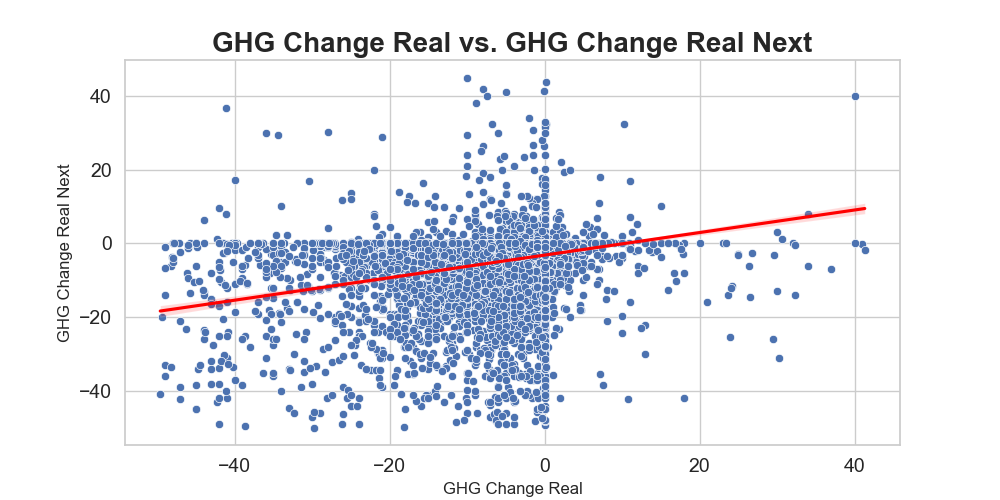
\includegraphics[width=\textwidth]{figures/ghg_change_real_vs_ghg_change_real_next.png}
\caption{Current vs. Next Year Decarbonization Rate}
\label{fig:ghg_change_real_vs_ghg_change_real_next}
\end{figure}

\begin{figure}[H]
\centering
  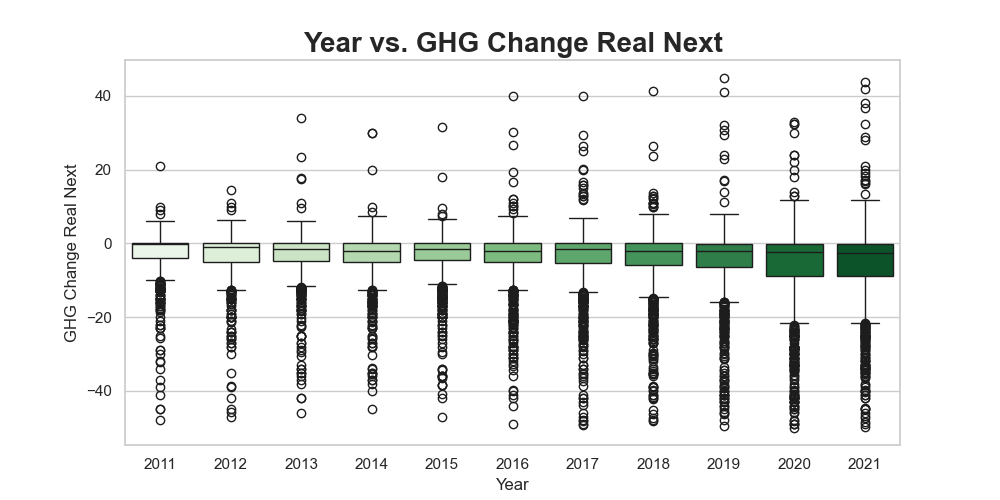
\includegraphics[width=\textwidth]{figures/year_vs_ghg_change_real_next.png}
\caption{Next Year Decarbonization Rate Over Time}
\label{fig:ghg_change_real_vs_year}
\end{figure}

    


\subsection{Discussion}
\begin{itemize}
    \item In model (1) from Table \ref{tab:R1}, we start by predicting \textit{Next-Year Decarbonization Rate} using year and Same-Year Decarbonization Rate. We observe how on average we predict a 22\% decrease in real decarbonization rate, as well as a positive and significant correlation between previous year and next year decarbonization rate. In particular, controlling for year, an increase in decarbonization rate from the previous year corresponds to 0.3 predicted next year increase in decarbonization rate. The marginal relationship between Same-Year Decarbonization Rate and Next-Year decarboninzation rate can be observed in Figure \ref{fig:ghg_change_real_vs_ghg_change_real_next}, where we observe a positive correlation. Analogously, the relationship between year and the response variable is presented in Figure \ref{fig:ghg_change_real_vs_year} where we observe that over time the variance of decarboninzation rates increases, while the mean slightly decreases.
    \item In model (2) from Table \ref{tab:R1}, we add our first random effect: a random intercept for the firm unique identifier code. Mixed effect models are particularly suited when we have repeated measures on the same individuals, in our case, the same firms. In particular, including an effect for each individual firm allows to take into account the correlation between each firm's timeseries without introducing an excessively high number of parameters. When adding Id as a random effect, the model's AIC decreases from 94134.242 to 94018.79, signaling a significant improvement in the model's fit. Furthermore, the signs of the coefficient yeear and ghg change real remain the same, and the coefficient for year remains significant. 
    \item \textbf{Key Finding:} Adding a random effect significantly improves the model's fit, and we will therefore iterate to find the optimal combination of random effects to then identify a comprehensive set of fixed effects that best predict decarbonization rates. 
\end{itemize}






\section{Model II: Impact of Industry Sector on Next-Year Decarbonization Rate}

\subsection{Key Hypothesis:}
\begin{itemize}
    \item Does the industry sector significantly influence the next year's decarbonization rate?
    \item Are there inherent differences in the decarbonization rates across different sectors due to their varying carbon-intensive natures?
    \item By introducing the industry as a random effect nested within firm IDs, does the model better capture the variances in decarbonization rates across different firms and industries?
\end{itemize}

\subsection{Models} 
\begin{enumerate}
    \item Linear Mixed Effect Model incorporating firm Id as a random intercept and including Industry as a fixed effect.
    \item Linear Mixed Effect Model incorporating Industry as a random effect nested within firm ID, along with the same fixed effects as model (1).
\end{enumerate}



% \subsection{Model II: Impact of Industry Sector on Next-Year Decarbonization Rate}
% \begin{itemize}
% \item In model (1) from table \ref{tab:../../thesis_tex/tables/R2.tex}, we add an important categorical predictor: industry. As explained in the EDA, Industry is derived using the Global Industry Classification stantard and it comprehends 20 industry categories. The hypothesis we want to test is whether the industry a firm operates in significantly affects decarbonization rate, and I expect the result to show that it does. We chose as reference category the Software, Services industry, which is the category that corresponds to the lowest (best) mean decarbonization rate. In this way, coefficients of other industries are expected to be positive and will represent the difference in decarbonization rate compared to the reference category.
% \item As we can observe from the Table, when controlling for year and previous year decarbonization rate, and having firm Id as a random effect, almost all industry sectors are significant, and the results are in line with what we found in the Exploratory Data Analysis section. In particular, sectors that displayed a higher (worse) mean decarbonization rates, such as the Energy, Materials, and Transportation sectors, have higher coefficients. Therefore, the model predicts that firms in these sectors will have a lower next-year decarbonization rate compared to the reference category. This makes sense as these sectors are known to be more carbon-intensive, and the model suggests that the carbon-intensive nature holds true even when controlling for time  and previous year decarbonization rate. We can infer that there likely are factor that make a sector inherently difficult to decarbonize. An example to support this finding is the case of decarbonizing cement production, which is a key category in the Material sector and contributes to a significant portion of global emissions. Cement production is inherently carbon-intensive, and the industry has been struggling to find a viable alternative to the traditional production process. This is a clear example of how the industry a firm operates in can significantly affect its decarbonization rate.
% \item The fact that firms Ids are nested into sector, as each firm is assigned to a primary GICS sector, allows to add Industry as a random effect on the model, nested into firm Id. The implementation is shown in model (2) from table \ref{tab:../../thesis_tex/tables/R2.tex}, and although there is an increase in the AIC, the coefficients for \textit{Year} and \textit{Ghg Change Real} remain significant and with the same sign and similar magnitude. 
% \end{itemize}

% \textbf{Key takeaways}:
% \begin{itemize}
%     \item The industry a firm operates in significantly affects its decarbonization rate, and the effect holds true even when controlling for time and previous year decarbonization rate.
%     \item The fact that firms Ids are nested into sector, as each firm is assigned to a primary GICS sector, allows to add Industry as a random effect on the model, nested into firm Id. From now on, we will include industry as a random effect in all the following models.
% \end{itemize}

\begin{table}[H] \centering    \caption{Model Comparison: Fixed Effects Only vs. Random Intercept for Firm Id and Industry}    \label{tab:../../thesis_tex/tables/R2.tex}  \resizebox{\textwidth}{!}{\begin{tabular}{@{\extracolsep{5pt}}lcc}  \\[-1.8ex]\hline  \hline \\[-1.8ex]   & \multicolumn{2}{c}{\textit{Dependent variable:}} \\  \cline{2-3}  \\[-1.8ex] & \multicolumn{2}{c}{Next Year Decarbonization Rate} \\  \\[-1.8ex] & \multicolumn{2}{c}{\textit{linear}} \\   & \multicolumn{2}{c}{\textit{mixed-effects}} \\  \\[-1.8ex] & (1) & (2)\\  \hline \\[-1.8ex]   Year & $-$0.260$^{***}$ (0.021) & $-$0.259$^{***}$ (0.021) \\    Ghg.Change.Real & 0.206$^{***}$ (0.009) & 0.209$^{***}$ (0.009) \\    IndustryAutomobiles, Components & 3.851$^{***}$ (0.631) &  \\    IndustryBanks & 1.870$^{***}$ (0.568) &  \\    IndustryCapital Goods & 3.347$^{***}$ (0.519) &  \\    IndustryCommercial, Professional Services & 4.121$^{***}$ (0.645) &  \\    IndustryConsumer Durables, Apparel & 2.356$^{***}$ (0.631) &  \\    IndustryConsumer Services & 3.528$^{***}$ (0.715) &  \\    IndustryConsumer Staples Distribution, Retail & 3.216$^{***}$ (0.698) &  \\    IndustryEnergy & 4.069$^{***}$ (0.592) &  \\    IndustryEquity Real Estate Investment Trusts & 1.207$^{*}$ (0.656) &  \\    IndustryFinancial Services & 2.591$^{***}$ (0.607) &  \\    IndustryFood, Beverage, Tobacco & 3.452$^{***}$ (0.574) &  \\    IndustryHealth Care Equipment, Services & 3.062$^{***}$ (0.653) &  \\    IndustryHousehold, Personal Products & 1.674$^{**}$ (0.797) &  \\    IndustryInsurance & 2.519$^{***}$ (0.617) &  \\    IndustryMaterials & 4.475$^{***}$ (0.522) &  \\    IndustryMedia, Entertainment & 2.226$^{***}$ (0.779) &  \\    IndustryPharmaceuticals, Biotechnology, Life Sciences & 2.721$^{***}$ (0.626) &  \\    IndustryReal Estate Management, Development & 2.227$^{**}$ (0.874) &  \\    IndustryRetailing & 1.527$^{**}$ (0.683) &  \\    IndustrySemiconductors, Semiconductor Equipment & 3.585$^{***}$ (0.702) &  \\    IndustryTechnology Hardware, Equipment & 2.381$^{***}$ (0.614) &  \\    IndustryTelecommunication Services & 1.770$^{***}$ (0.657) &  \\    IndustryTransportation & 3.754$^{***}$ (0.605) &  \\    IndustryUtilities & 3.487$^{***}$ (0.562) &  \\    Constant & $-$5.196$^{***}$ (0.484) & $-$2.395$^{***}$ (0.241) \\   \hline \\[-1.8ex]  \textbf{Random Effects:} &  &  \\  Number of Firms & 1870 & 1870 \\  Number of Industries &  & 25 \\  sd(Firms) & 1.953 & 1.93 \\  sd(Industry) &  & 0.972 \\  Akaike Inf. Crit. & 93891.439 & 93919.569 \\  Bayesian Inf. Crit. & 94109.755 & 93964.738 \\  \hline  \hline \\[-1.8ex]  \textit{Note:}  & \multicolumn{2}{r}{$^{*}$p$<$0.1; $^{**}$p$<$0.05; $^{***}$p$<$0.01} \\   & \multicolumn{2}{r}{Second model has firm Id and Industry as random intercepts.} \\  \end{tabular}}  \end{table} 

\subsection{Relevant Figures:}

\begin{figure}[H]
\centering
  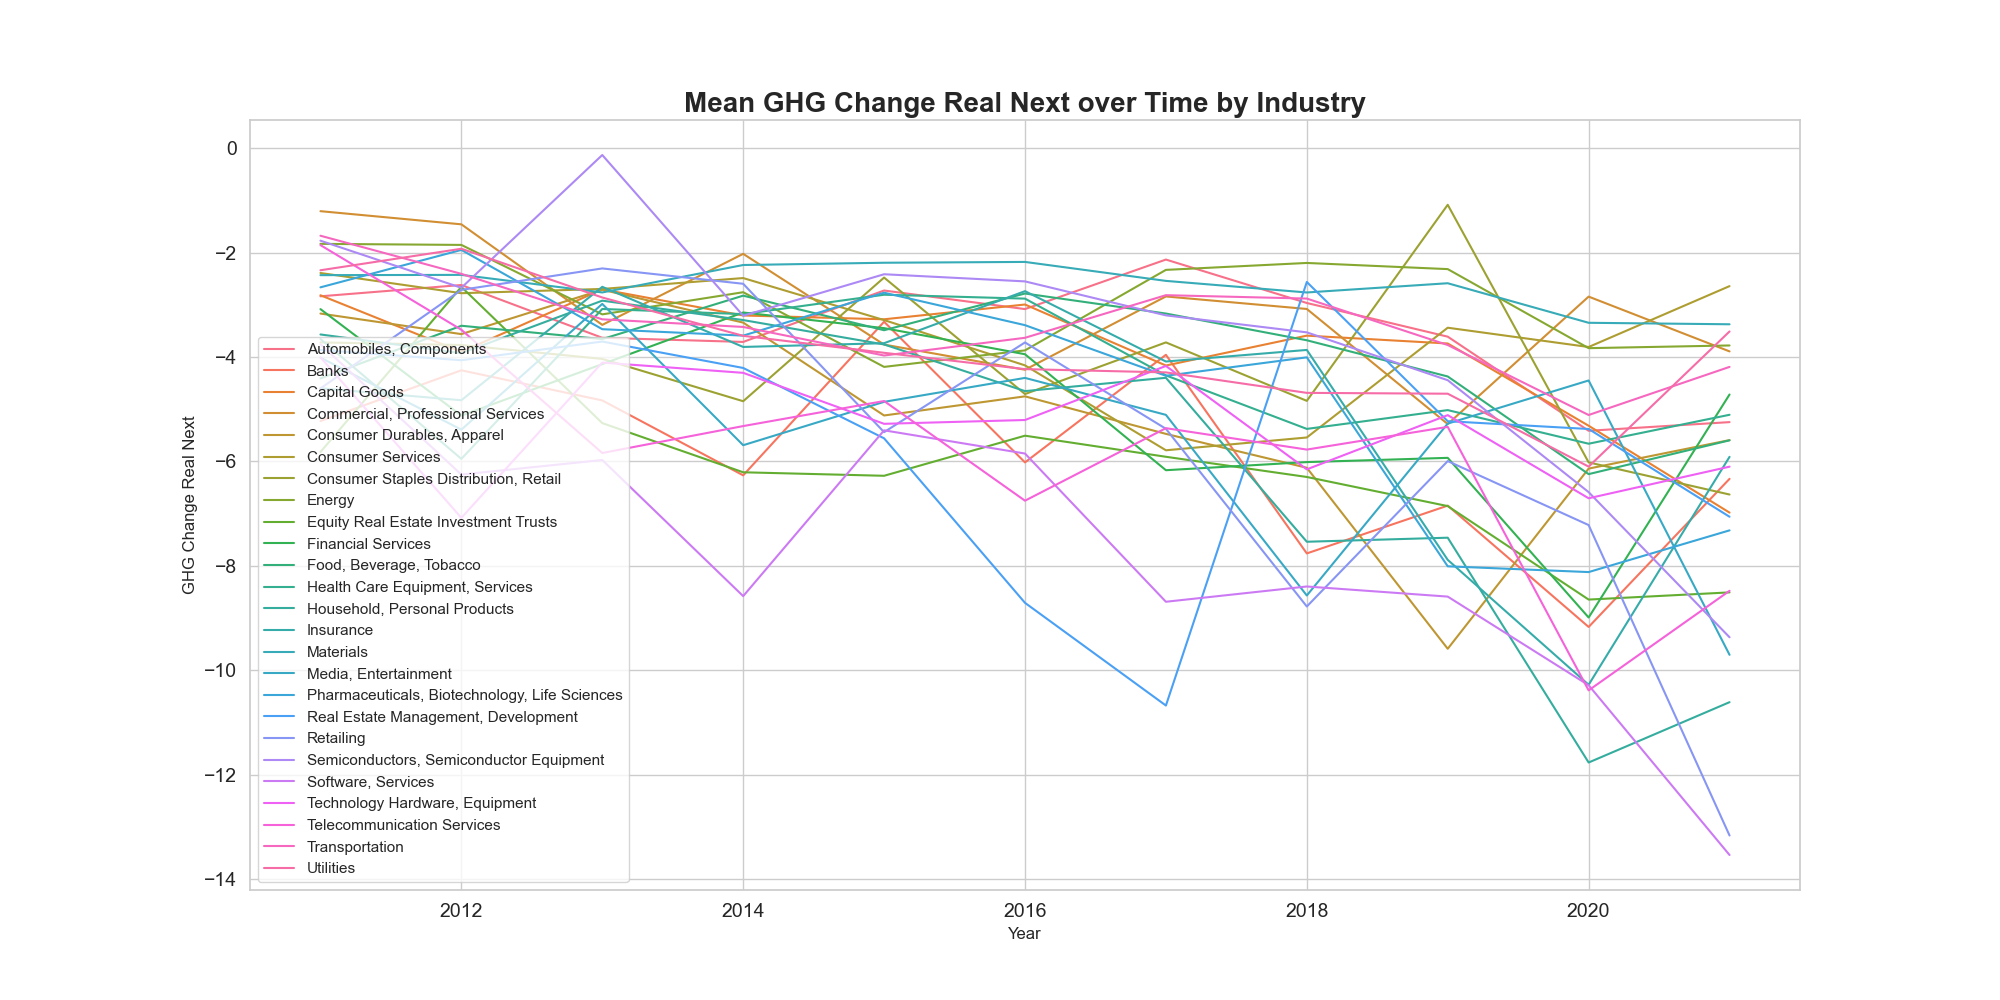
\includegraphics[width=\textwidth]{figures/ghg_change_real_next_over_time_by_industry.png}
\caption{Next Year Decarbonization Rate by Industry}
\label{fig:industry_vs_ghg_change_real_next}
\end{figure}

\subsection{Discussion}
\begin{itemize}
    \item In model (1), the inclusion of industry sector as a categorical predictor provides a clear indication that the decarbonization rate is significantly influenced by the sector in which a firm operates. The coefficients from the model suggest that, compared to the Software, Services industry (reference category), firms in sectors like Energy, Materials, and Transportation have significantly higher decarbonization rates, aligning with the expectation due to their carbon-intensive nature.
    \item Model (2) incorporates industry sector as a random effect nested within firm IDs, accounting for the non-independence of observations within the same sector and firm. This model variation reflects the hierarchical structure of data. Despite an increase in AIC, indicating a more complex model, the significant predictors remain consistent, suggesting that industry can be effectively used as a random effect.
    \item The mean decarboninzation trends by industry are presented in Figure \ref{fig:industry_vs_ghg_change_real_next}. We can observe that over time mean decarboninzation rates are improving (decreasing) and that some industries tend to decarbonize more than others as expected.
    \item \textbf{Key Finding:} The significant effect of the industry sector on decarbonization rates underscores the importance of considering sector-specific factors when evaluating environmental performance. The persistence of significant coefficients for industry sectors across both models indicates that certain industries face inherent challenges in reducing carbon emissions. This could be due to technological barriers, regulatory differences, economic constraints, or the fundamental carbon intensity of their operations. Overall, the addition of industry as a random effect nested within firm IDs in Model (2) helps to better capture the intra-sector variability and the unique characteristics of firms. While this increases model complexity, as evidenced by the higher AIC, it provides a more accurate representation of the real-world scenario where firms within the same industry may follow different decarbonization trajectories due to various factors such as size, location, and management practices.
    
\end{itemize}

% \begin{itemize}
%     \item A predictor we will next consider is georgraphical location. Location is important in understanding decarbonization rates, as different countries have different policies and regulations that can affect a firm's ability to decarbonize. 
%     \item In model (1) from Table \ref{tab:R3}, we start by predicting \textit{Next-Year Decarbonization Rate} using year, ghg change real, and continent. Our reference category is Europe, and we expect the coefficients for the other continents to be positive, as we expect firms in other continents to have a lower decarbonization rate compared to firms in Europe. The results are in line with our expectations, and all coefficients are significant.
%     \item In model (2) from Table \ref{tab:R3}, we add country as a random effect, nested into continent. The AIC increases, but the coefficients for year and ghg change real remain significant and with the same sign and identical magnitude. This is a good sign, and it suggest that our panel data can be effectively modeled using a mixed effect model with firm Id, industry, and country nested into continent as random effects.
%     \item \textbf{Key Finding:} The continent a firm is located in is significantly associated with its decarbonization rate, and the effect holds true even when controlling for time and previous year decarbonization rate and having firm Id and industry as random effects. Furthermore, adding country nested into continent as a random effect does not significantly change the model's fit, and we will therefore include it in all the following models.
% \end{itemize}

\section{Model III: Impact of Country and Continent on Next-Year Decarbonization Rate}

\subsection{Key Hypothesis}
\begin{itemize}
    \item How does a firm's geographical location, specifically its continent and country, impact its decarbonization rate?
    \item Given the different environmental policies, economic conditions, and technological advancements across countries, can these geographical differences explain variations in decarbonization rates?
    \item Will the addition of geographical variables as random effects nested within each other improve the model's ability to explain variations in decarbonization rates among firms?
\end{itemize}

\subsection{Models} 
\begin{enumerate}
    \item Linear Mixed Effect Model incorporating Year, GHG Change Real, and Continent as fixed effects, and firm ID and industry as random intercepts.
    \item Linear Mixed Effect Model adding Country as a random effect nested within Continent, in addition to the fixed and random effects included in model (1).
\end{enumerate}

\begin{table}[H] \centering    \caption{Impact of Country and Continent on Next-Year Real Decarbonization Rate}    \label{tab:R3}  \resizebox{0.8\textwidth}{!}{\begin{tabular}{@{\extracolsep{5pt}}lcc}  \\[-1.8ex]\hline  \hline \\[-1.8ex]   & \multicolumn{2}{c}{\textit{Dependent variable:}} \\  \cline{2-3}  \\[-1.8ex] & \multicolumn{2}{c}{Next Year Decarbonization Rate} \\  \\[-1.8ex] & (1) & (2)\\  \hline \\[-1.8ex]   Year & $-$0.267$^{***}$ (0.021) & $-$0.267$^{***}$ (0.021) \\    Ghg.Change.Real & 0.207$^{***}$ (0.009) & 0.207$^{***}$ (0.009) \\    ContinentAfrica & 1.895$^{***}$ (0.409) &  \\    ContinentAsia & 1.714$^{***}$ (0.202) &  \\    ContinentNorth America & 1.377$^{***}$ (0.185) &  \\    ContinentOceania & 1.585$^{***}$ (0.519) &  \\    ContinentSouth America & 1.058$^{**}$ (0.524) &  \\    Constant & $-$3.282$^{***}$ (0.258) & $-$2.027$^{***}$ (0.413) \\   \hline \\[-1.8ex]  \textbf{Random Effects:} &  &  \\  Number of Firms & 1871 & 1871 \\  Number of Industries & 25 & 25 \\  Number of Continents & 6 & 6 \\  Number of Countries &  & 48 \\  sd(Firms:Industry) & 1.789 & 1.766 \\  sd(Industry) & 0.975 & 0.97 \\  sd(Continent) &  & 0.74 \\  sd(Country:Continent) &  & 0.349 \\  Akaike Inf. Crit. & 93831.892 & 93834.542 \\  Bayesian Inf. Crit. & 93914.702 & 93894.767 \\  \hline  \hline \\[-1.8ex]  \textit{Note:}  & \multicolumn{2}{r}{$^{*}$p$<$0.1; $^{**}$p$<$0.05; $^{***}$p$<$0.01} \\ \multicolumn{3}{p{\textwidth}}{\textit{Model (1): Linear Mixed Effect Model incorporating Year, GHG Change Real, and Continent as fixed effects, and firm ID and industry as random intercepts. Model (2): Linear Mixed Effect Model adding Country as a random effect nested within Continent, in addition to the fixed and random effects included in model (1).}}
\end{tabular}}  \end{table} 

\subsection{Relevant Figures:}

\begin{figure}[H]
\centering
  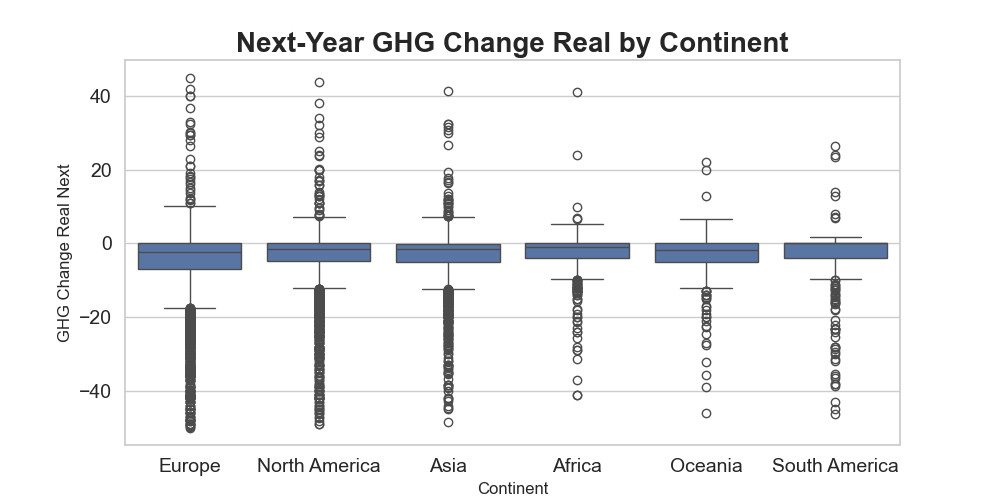
\includegraphics[width=\textwidth]{figures/ghg_change_real_next_by_continent.png}
\caption{Continent vs. Next Year Decarbonization Rate}
\label{fig:continent_vs_ghg_change_real_next}
\end{figure}

\subsection{Discussion}
\begin{itemize}
    \item Model (1) introduces the effect of geographical location at the continental level as a fixed effect while controlling for year and GHG change, and using firm ID and Industry as random intercepts. The significant coefficients for continents compared to Europe (the reference category) suggests that geographical location is correlated with a significant change firm's decarbonization rate, in particular we observe how Oceania is the continent associated with the least decarbonization. That is, compared to Europe, according to the model a firm in Oceana is predicted to decarbonize by an average of $1.585 \%$ less compared to Europe. This finding aligns with expectations, reflecting variations in regulatory environments, access to clean technologies, and economic conditions across continents. A comparison between continents is also provided in Figure \ref{fig:continent_vs_ghg_change_real_next}, where we observe how Europe's distribution is centered around a lower mean compared to other continents. 
    \item Model (2) incorporates country as a random effect nested within continents. This allows to take into account the effect of geographical location in future models without increasing the degrees of freedom. Although the AIC slightly increases, indicating a more complex model, the consistency of significant coefficients for Year and GHG Change Real across both models suggests that these are robust predictors of decarbonization rates.
    \item \textbf{Key Finding:} The analysis demonstrates that the continent and country where a firm is located significantly impact its decarbonization rate, highlighting the importance of geographical factors in environmental strategies. Moving forward, the inclusion of country and continent as significant variables will be included in all subsequent models. Form now on, the random effects will always be the same: that is random intercepts for firm Id nested wihtin Industry, and random intercepts for Country nested wihtin Continent. 
\end{itemize}

 

\section{Model IV: Impact of Financial Predictors on Next-Year Decarbonization Rate}

\subsection{Key Hypothesis}
\begin{itemize}
    \item How do financial predictors such as market capitalization, revenue, and growth in assets and employees affect a firm's decarbonization rate?
    \item Is there a correlation between a firm's size, as measured by market cap and revenue, and its ability or effort to decarbonize?
    \item How do factors indicative of a firm's growth, such as growth in assets and employees, correlate with its decarbonization rate?
\end{itemize}

\subsection{Models} 
\begin{enumerate}
    \item Linear Mixed Effect Model evaluating the impact of Year, GHG Change Real, Market Cap, and Revenue on Next-Year Decarbonization Rate, with Firm ID and Industry as random intercepts.
    \item Extension of Model (1) adding Assets Growth as an additional predictor.
    \item Further extension of Model (2) adding Employees Growth as an additional predictor.
\end{enumerate}

\begin{table}[H] \centering    \caption{Financial Predictors vs. Next Year Real Decarbonization Rate}    \label{tab:R4}  \resizebox{0.8\textwidth}{!}{\begin{tabular}{@{\extracolsep{5pt}}lccc}  \\[-1.8ex]\hline  \hline \\[-1.8ex]   & \multicolumn{3}{c}{\textit{Dependent variable:}} \\  \cline{2-4}  \\[-1.8ex] & \multicolumn{3}{c}{Next Year Decarbonization Rate} \\  \\[-1.8ex] & (7) & (8) & (9)\\  \hline \\[-1.8ex]   Year & $-$0.258$^{***}$ (0.021) & $-$0.256$^{***}$ (0.021) & $-$0.256$^{***}$ (0.021) \\    Ghg.Change.Real & 0.204$^{***}$ (0.009) & 0.205$^{***}$ (0.009) & 0.205$^{***}$ (0.009) \\    Market.Cap & $-$0.405$^{***}$ (0.115) & $-$0.520$^{***}$ (0.088) & $-$0.529$^{***}$ (0.089) \\    Employees & 0.047 (0.093) &  &  \\    Revenue & 0.234 (0.156) & 0.154$^{*}$ (0.091) & 0.162$^{*}$ (0.092) \\    Employees.1Y.Gr & $-$0.024 (1.222) & 0.489 (1.070) &  \\    Assets.1Y.Gr & 1.020 (1.099) &  & 0.791 (0.954) \\    Tot.Assets & $-$0.225 (0.138) &  &  \\    Net.Income.Over.Assets & $-$2.597 (4.659) &  &  \\    Roe & $-$0.662 (1.239) &  &  \\    Constant & 8.158$^{**}$ (3.222) & 5.854$^{***}$ (1.605) & 5.618$^{***}$ (1.573) \\   \hline \\[-1.8ex]  \textbf{Random Effects:} &  &  &  \\  Number of Firms & 1871 & 1871 & 1871 \\  Number of Industries & 25 & 25 & 25 \\  Number of Continents & 6 & 6 & 6 \\  Number of Countries & 48 & 48 & 48 \\  sd(Firms:Industry) & 1.733 & 1.729 & 1.729 \\  sd(Industry) & 0.898 & 0.899 & 0.898 \\  sd(Continent) & 0.74 & 0.746 & 0.745 \\  sd(Country:Continent) & 0.275 & 0.274 & 0.277 \\  Akaike Inf. Crit. & 93831.892 & 93834.542 & 93793.357 \\  Bayesian Inf. Crit. & 93914.702 & 93894.767 & 93913.807 \\  \hline  \hline \\[-1.8ex]  \textit{Note:}  & \multicolumn{3}{r}{$^{*}$p$<$0.1; $^{**}$p$<$0.05; $^{***}$p$<$0.01} \\ \multicolumn{4}{p{\textwidth}}{\textit{Model (7): Linear Mixed Effect Model evaluating the impact of Year, GHG Change Real, Market Cap, and Revenue on Next-Year Decarbonization Rate, with Firm ID and Industry as random intercepts. Model (8): Extension of Model (7) adding Assets Growth as an additional predictor. Model (9): Further extension of Model (8) adding Employees Growth as an additional predictor.}} \\  \end{tabular}}  
\end{table} 

\subsection{Relevant Figures:}
\begin{figure}[H]
\centering
  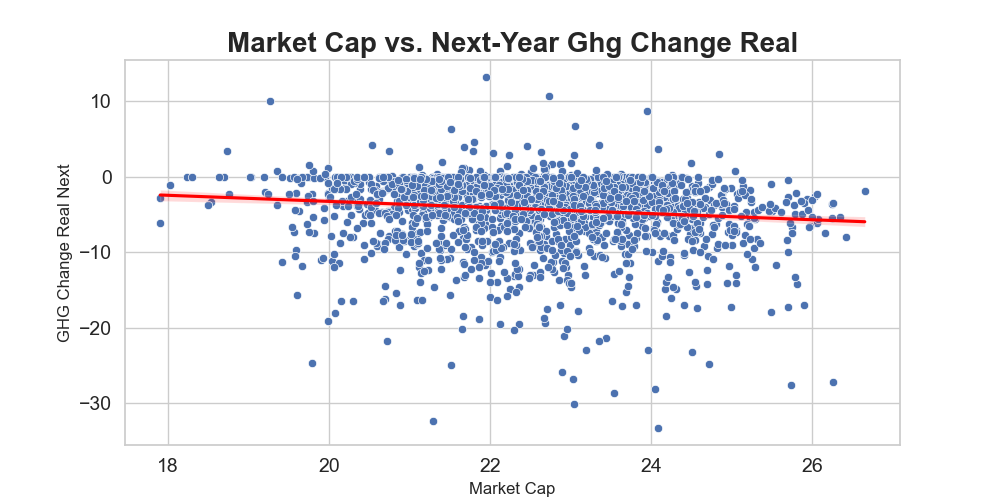
\includegraphics[width=\textwidth]{figures/market_cap_vs_ghg_change_real_next.png}
\caption{Market Capitalization vs. Next Year Decarbonization Rate}
\label{fig:market_cap_vs_ghg_change_real_next}
\end{figure}

\begin{figure}[H]
\centering
  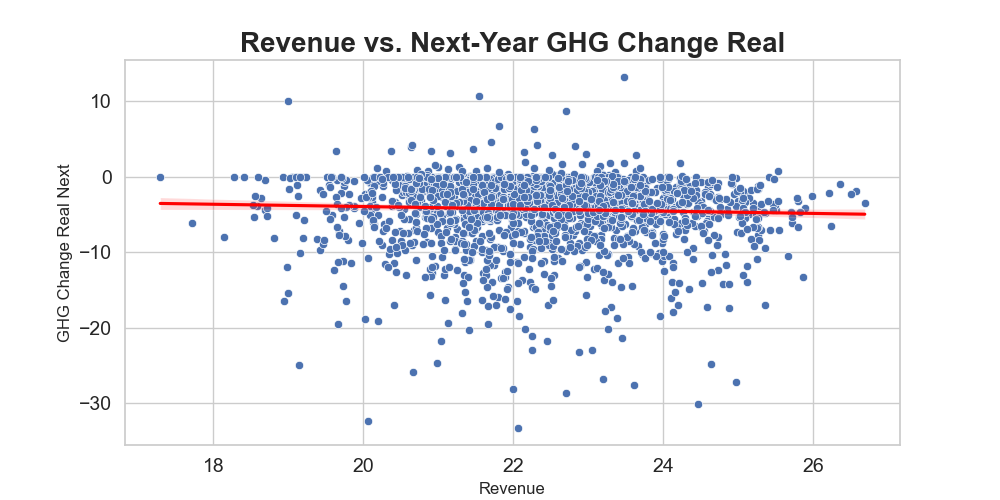
\includegraphics[width=\textwidth]{figures/revenue_vs_ghg_change_real_next.png}
\caption{Revenue vs. Next Year Decarbonization Rate}
\label{fig:revenue_vs_ghg_change_real_next}
\end{figure}

\subsection{Discussion}
\begin{itemize}
    \item In Model (1), significant predictors include Year, GHG Change Real, and Market Cap, with Revenue showing significance at the 10\% level. The negative coefficient for Market Cap suggests that larger firms have a lower, which in this context means better, decarbonization rate. The marginal relationship is presented in Figure \ref{fig:market_cap_vs_ghg_change_real_next} where we can clearly observe a negative correlation between market cap and decarbonization rate. A similar, though less pronounced marginal relationship also applies to revenuue, as can be observed in Figure \ref{fig:revenue_vs_ghg_change_real_next}.
    
    \item Model (2) focuses on Assets Growth as a variable, controlling for Market Cap and Revenue and removing other non-significant predictors. The positive but non-significant coefficient for Assets Growth suggests an expected correlation relationship where firms expanding their assets might experience a worse rate of decarbonization, potentially due to increased operations or capital investment not directly tied to reducing emissions. 
    
    \item Model (3) includes Employees Growth, which also shows a non-significant result. Similar to Assets Growth, the positive direction of the Employees Growth coefficient hints at a conceivable relationship where firms increasing their workforce may not proportionally enhance their decarbonization efforts. Yet, this remains speculative without statistical significance. 
    
    \item \textbf{Key Finding:} Financial indicators, particularly Market Cap and, to a lesser extent, Revenue, serve as relevant predictors for a firm's decarbonization rate. The consistent significance and direction of these coefficients across models suggest a potential link between a firm's financial scale and its environmental performance. Financial metrics will continue to be used as control variables in future models to refine our understanding of their impact on decarbonization rates. The positive but non significant coefficients of growth indicators in my opinion hint at the fact that it is challenging to grow and decarbonize at the same time.
\end{itemize}




% \subsection{Impact of Financial Predictors on Decarbonization}

% \begin{itemize}
%     \item In model (1) from Table \ref{tab:R4}, we start by predicting \textit{Next-Year Decarbonization Rate} using year, ghg change real, market cap, employees, and revenue, employees 1 year growth, assets 1 year growth, total assets, net income over assets, and return on equity. We find that only market cap is significant, with revenue being significant at the 10\% level. The coefficient for market cap is negative, and the coefficient for revenue is positive. This is in line with our expectations, as we expect larger firms to have a more negative (higher) decarbonization rate, and we expect firms with higher revenue to have a less negative (lower) decarbonization rate. Since the revenue coefficient is not significant at the 5\% level, and there are many omitted variables that could be affecting the results, we will not draw any conclusions from this model. We will focus on retaining both market cap and revenue in the next model, and we will focus on understanding how assets and empllyees growth affect next year decarbonization rate in the following model.
%     \item In model (2) from Table \ref{tab:R4}, we add assets growth. We find that assets growth is not significant, and the coefficients for market cap and revenue remain significant and with the same sign and similar magnitude. Although not significant, the coefficient for assets growth is positive, which seems to suggest that firms with higher assets growth have a lower decarbonization rate.
%     \item In model (3) from Table \ref{tab:R4}, we add employees growth. We find that employees growth is not significant, and the coefficients for market cap and revenue remain significant and with the same sign and similar magnitude. Employees growth is positive, which seems to suggest that firms with higher employees growth have a lower decarbonization rate. 
%     \item \textbf{Key Finding:} Market cap and revenue provide useful information on a firm's decarbonization rate. It seems that firms with higher revenue and employees growth have a lower decarbonization rate, and firms with a high market cap have a higher decarbonization rate. I would not draw conclusions based solely on financial predictors, as it could be the case that they are capturing the effect of other omitted variables. They serve as useful control variables, and we will therefore include them in all the following models.
% \end{itemize}



\section{Model V: Impact of GHG Emissions and Verification on Next-Year Decarbonization Rate}

\subsection{Key Hypothesis}
\begin{itemize}
    \item How do different scopes of greenhouse gas emissions and their verification statuses influence a firm's decarbonization rate?
    \item Are there metrics on a specific emission scope that are more significant predictors of decarbonization rates than analogous metrics on other scopes?
    \item Does the verification of GHG emissions have a significant impact on the firm's decarbonization efforts?
\end{itemize}

\subsection{Models}
\begin{enumerate}
    \item First model: Includes all predictors in the set and analyzes all hypothesis: how different greenhouse gas (GHG) emissions, whether they're checked (verified), and other basic company details like size and earnings, affect how much a company can reduce its emissions in a year.
    \item Second model: Just focuses on the types of GHG emissions to see which ones are most important for reducing emissions, still considering basic company details.
    \item Third model: Only looks at whether companies check (verify) their emissions data and how that influences their ability to cut down emissions, keeping the company details the same.
    \item Fourth model: Picks out and uses only the most important factors from the first three models, those predictors will be passed on in the next models.
\end{enumerate}

\begin{table}[H] \centering    \caption{Emission and Verification vs. Next Year Decarbonization Rate}    \label{tab:R5}  \resizebox{0.8\textwidth}{!}{\begin{tabular}{@{\extracolsep{5pt}}lcccc}  \\[-1.8ex]\hline  \hline \\[-1.8ex]   & \multicolumn{4}{c}{\textit{Dependent variable:}} \\  \cline{2-5}  \\[-1.8ex] & \multicolumn{4}{c}{Next Year Decarbonization Rate} \\  \\[-1.8ex] & (10) & (11) & (12) & (13)\\  \hline \\[-1.8ex]   Year & $-$0.118$^{***}$ (0.028) & $-$0.211$^{***}$ (0.022) & $-$0.111$^{***}$ (0.028) & $-$0.111$^{***}$ (0.027) \\    Ghg.Change.Real & 0.198$^{***}$ (0.009) & 0.200$^{***}$ (0.009) & 0.196$^{***}$ (0.009) & 0.196$^{***}$ (0.009) \\    Market.Cap & $-$0.438$^{***}$ (0.087) & $-$0.447$^{***}$ (0.087) & $-$0.403$^{***}$ (0.086) & $-$0.409$^{***}$ (0.086) \\    Revenue & 0.183$^{*}$ (0.099) & 0.246$^{***}$ (0.090) & 0.204$^{**}$ (0.098) & 0.176$^{*}$ (0.095) \\    Ghg1 & 0.107$^{***}$ (0.037) &  & 0.126$^{***}$ (0.037) & 0.115$^{***}$ (0.035) \\    Ghg2Location & $-$0.087$^{**}$ (0.042) &  & $-$0.088$^{**}$ (0.042) & $-$0.066$^{***}$ (0.025) \\    Ghg2Market & $-$0.016 (0.031) &  & $-$0.022 (0.031) &  \\    Ghg3.Total & $-$0.032 (0.020) &  & $-$0.015 (0.020) &  \\    Ghg3.Count & $-$0.086$^{***}$ (0.030) &  & $-$0.058$^{*}$ (0.030) & $-$0.073$^{***}$ (0.024) \\    Ghg1.Na & 1.732$^{***}$ (0.583) &  & 1.845$^{***}$ (0.586) & 1.682$^{***}$ (0.507) \\    Ghg2Location.Na & $-$0.324 (0.580) &  & $-$0.396 (0.578) &  \\    Ghg2Market.Na & 0.886$^{**}$ (0.358) &  & 0.767$^{**}$ (0.358) & 0.991$^{***}$ (0.178) \\    Ghg3.Total.Na & 0.039 (0.437) &  & $-$0.010 (0.438) &  \\    Methane.Emissions & 0.078$^{***}$ (0.022) &  & 0.079$^{***}$ (0.022) & 0.077$^{***}$ (0.022) \\    Type.Scope1Limited/Moderate &  & 0.320 (0.225) & 0.367 (0.224) & 0.360 (0.221) \\    Type.Scope1N.A &  & 0.334 (0.450) & 0.629 (0.457) & 0.958$^{***}$ (0.263) \\    Type.Scope1Third.Party.Underway &  & 0.858$^{***}$ (0.299) & 0.807$^{***}$ (0.300) & 0.850$^{***}$ (0.295) \\    Ghg.Verification.Scope1.Yes &  & $-$0.444 (0.517) & $-$0.344 (0.528) &  \\    Ghg.Verification.Scope2.Yes &  & $-$0.317 (0.389) & $-$0.047 (0.391) &  \\    Ghg.Verification.Scope3.Yes &  & $-$0.610$^{***}$ (0.185) & $-$0.410$^{**}$ (0.190) & $-$0.458$^{**}$ (0.181) \\    Constant & 2.645$^{*}$ (1.543) & 2.732$^{*}$ (1.499) & 1.035 (1.602) & 1.000 (1.523) \\   \hline \\[-1.8ex]  \textbf{Random Effects:} &  &  &  &  \\  Number of Firms & 1871 & 1871 & 1871 & 1871 \\  Number of Industries & 25 & 25 & 25 & 25 \\  Number of Continents & 6 & 6 & 6 & 6 \\  Number of Countries & 48 & 48 & 48 & 48 \\  sd(Firms:Industry) & 1.617 & 1.643 & 1.588 & 1.58 \\  sd(Industry) & 0.704 & 0.857 & 0.649 & 0.648 \\  sd(Continent) & 0.671 & 0.689 & 0.644 & 0.637 \\  sd(Country:Continent) & 0.291 & 0.242 & 0.208 & 0.197 \\  Akaike Inf. Crit. & 93723.94 & 93738.237 & 93703.092 & 93683.497 \\  Bayesian Inf. Crit. & 93874.502 & 93858.688 & 93898.824 & 93834.06 \\  \hline  \hline \\[-1.8ex]  \textit{Note:}  & \multicolumn{4}{r}{$^{*}$p$<$0.1; $^{**}$p$<$0.05; $^{***}$p$<$0.01} \\  \multicolumn{5}{p{1.4\textwidth}}{\textit{Model (10): Includes all predictors in the set and analyzes all hypothesis: how different greenhouse gas (GHG) emissions, whether they're checked (verified), and other basic company details like size and earnings, affect how much a company can reduce its emissions in a year. Model (11): Just focuses on the types of GHG emissions to see which ones are most important for reducing emissions, still considering basic company details. Model (12): Only looks at whether companies check (verify) their emissions data and how that influences their ability to cut down emissions, keeping the company details the same. Model (13): Picks out and uses only the most important factors from the first three models, those predictors will be passed on in the next models.}} \\  \end{tabular}}  \end{table} 

\subsection{Relevant Figures:}
% first figure emission scope types
\begin{figure}[H]
\centering
  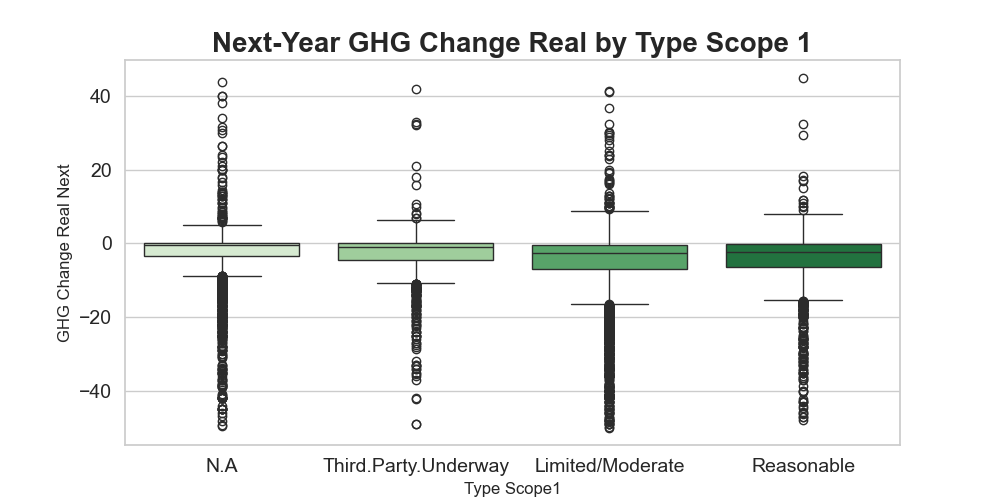
\includegraphics[width=\textwidth]{figures/ghg_change_real_next_by_type_scope1.png}
\caption{GHG Emission Scope 1 Verification Type vs. Next Year Decarbonization Rate}
\label{fig:ghg_change_real_next_by_ghg_type}
\end{figure}

% plot ghg1_vs_ghg_change_real_next
\begin{figure}[H]
\centering
    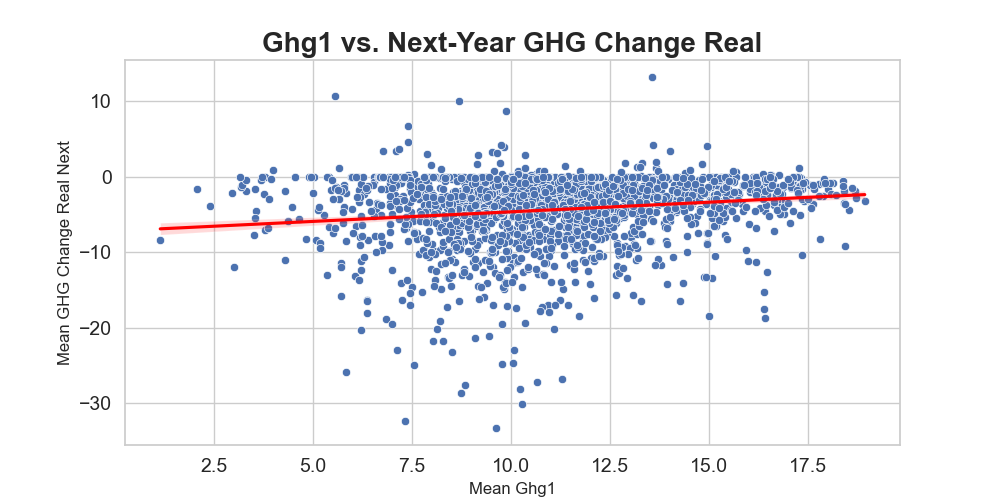
\includegraphics[width=\textwidth]{figures/ghg1_vs_ghg_change_real_next.png}
\caption{GHG Emission Scope 1 vs. Next Year Decarbonization Rate}
\label{fig:ghg1_vs_ghg_change_real_next}
\end{figure}

    

% second figure boxplot of Ghg1 Missing
\begin{figure}[H]
\centering
  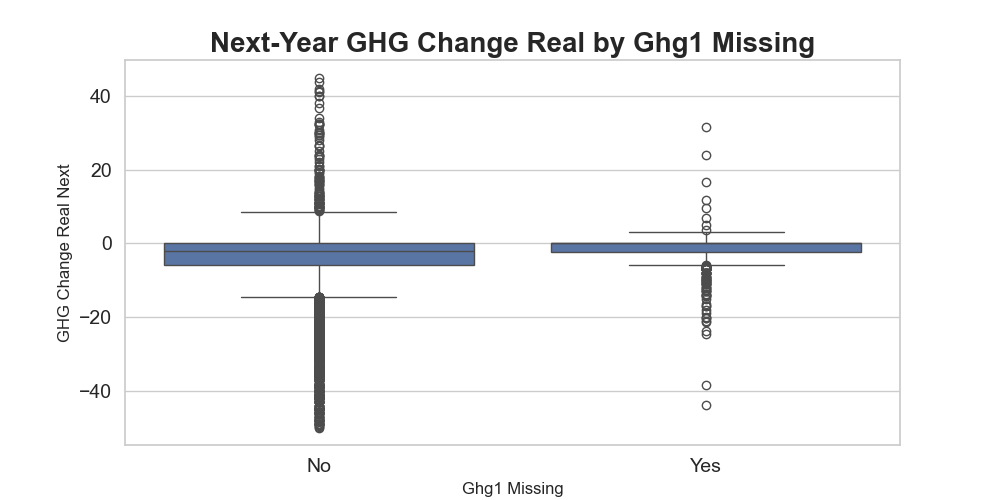
\includegraphics[width=\textwidth]{figures/ghg_change_real_next_by_ghg1_na.png}
\caption{GHG Emission Scope 1 Missing vs. Next Year Decarbonization Rate}
\label{fig:ghg_change_real_next_by_ghg1_na}
\end{figure}

% third figure scatter methane_emissions_vs_ghg_change_real_next
\begin{figure}[H]
\centering
  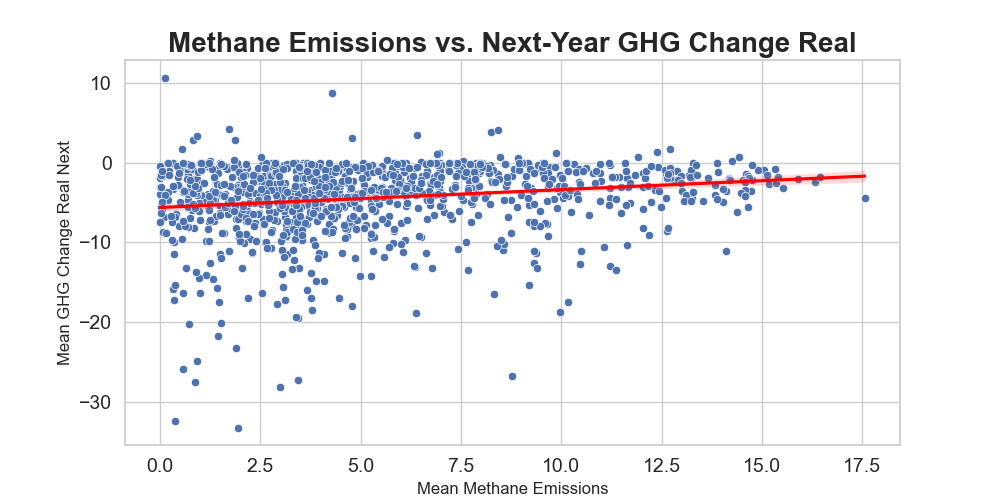
\includegraphics[width=\textwidth]{figures/methane_emissions_vs_ghg_change_real_next.png}
\caption{Methane Emissions vs. Next Year Decarbonization Rate}
\label{fig:methane_emissions_vs_ghg_change_real_next}
\end{figure}

% fourth figure is a boxplot of ghg_change_real_next_by_ghg2market_na
\begin{figure}[H]
\centering
  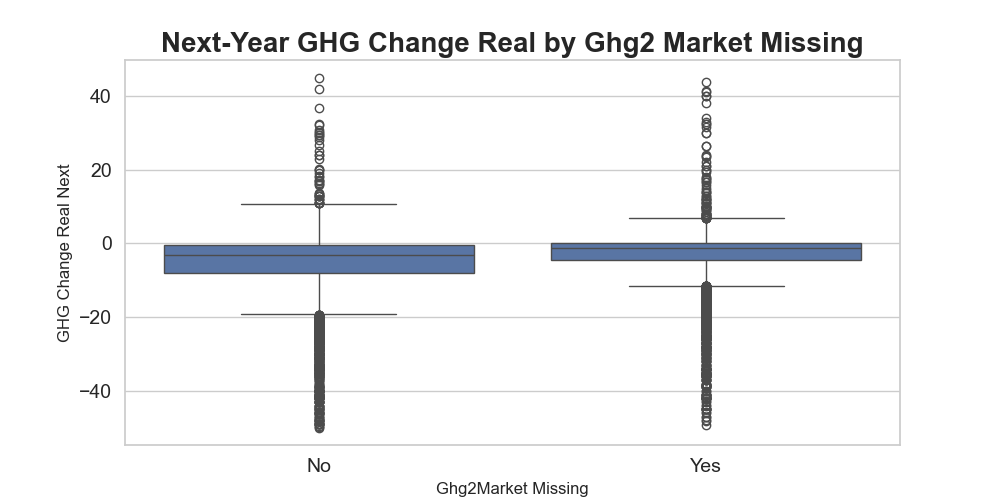
\includegraphics[width=\textwidth]{figures/ghg_change_real_next_by_ghg2market_na.png}
\caption{GHG Emission Scope 2 Market Missing vs. Next Year Decarbonization Rate}
\label{fig:ghg_change_real_next_by_ghg2market_na}
\end{figure}

% plot ghg_change_real_next_by_ghg_verification_scope3_yes
\begin{figure}[H]
\centering
  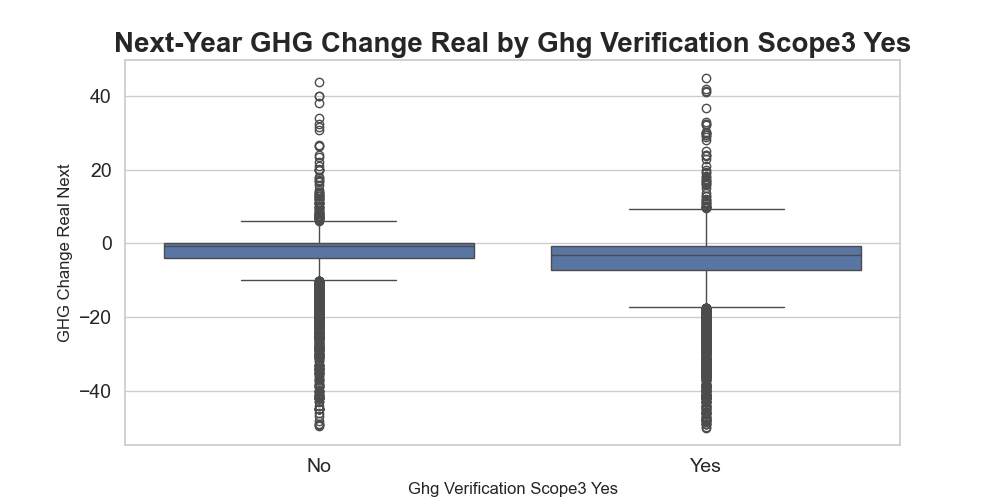
\includegraphics[width=\textwidth]{figures/ghg_change_real_next_by_ghg_verification_scope3_yes.png}
\caption{GHG Emission Scope 3 Verification vs. Next Year Decarbonization Rate}
\label{fig:ghg_change_real_next_by_ghg_verification_scope3_yes}
\end{figure}


\subsection{Discussion}

\begin{itemize}
    \item The analysis shows that Scope 1 emissions (Ghg1) significantly influence a firm's decarbonization efforts. A positive coefficient for Ghg1 (0.107, significant at the 1\% level) indicates that higher Scope 1 emissions are correlated with a poorer decarbonization rate for the next year. Furthermore, when data for Scope 1 emissions is missing (Ghg1.Na), there's a notable jump in the decarbonization rate, with a coefficient increase to 1.732. Specifically, firms that do not report their Scope 1 emissions are predicted to have a 0.577\% worse decarbonization rate compared to those that do report. This gap emphasizes the importance of accurate reporting; not reporting is linked to poorer environmental performance. The marginal relationship between Scope 1 emssions and Next-Year Decarbonization Rate is presented in Figure \ref{fig:ghg1_vs_ghg_change_real_next} where we observe that higer emissions are correlated with worse decarbonization rates. The relationship between reporting Scope 1 emissions is presented in the boxplot Figure \ref{fig:ghg_change_real_next_by_ghg1_na}.

    \item Regarding market emissions, the positive coefficient for not reporting market-based emissions (Ghg2Market.Na) is correlated with a predicted worse next-year decarbonizaiton rate by an average of $0.850 \%$. This makes sense since market-based reporting is more complex and firms that invest the effort likely prioritize decarbonization more strongly. The marginal relationship between reporting market-based emissions and the response is presented in Figure \ref{fig:ghg_change_real_next_by_ghg2market_na} where the firms that don't report have wrose decarboninzation rates on average.
    
    \item Methane emissions also play a significant role in the analysis. The presence of Methane Emissions with a positive coefficient ($0.078$, significant at the 1\% level) suggests that firms with higher reported methane emissions are expected to have a worse next-year decarbonization rate. This underlines the importance of focusing on specific pollutants like methane, which have a high impact on global warming and can significantly affect a firm's overall decarbonization performance. The marginal relationship between methane emissions and next-year decarboninzation rate is presented in Figure \ref{fig:methane_emissions_vs_ghg_change_real_next} where we observe a clear trend between firms with higher methane emissions having worse next-year decarboninzation rates.
    

    \item The role of emissions verification is also central in our findings, particularly the positive impact of verifying Scope 3 emissions. Firms that verify their Scope 3 emissions (Ghg.Verification.Scope3.Yes) are associated with a better decarbonization rate, with a negative coefficient of -0.610 (significant at the 1\% level in the second model and -0.458, significant at the 5\% level in the final model). The marginal relationship is presented in Figure \ref{fig:ghg_change_real_next_by_ghg_verification_scope3_yes}. This suggests that firms taking steps to validate their broadest category of emissions are likely more committed to comprehensive decarbonization efforts, as Scope 3 encompasses indirect emissions not produced by the firm directly but related to their value chain. Hence, verifying these emissions can be seen as an indication of a firm's comprhensive approach to understanding and mitigating its environmental impact.

    \item The type of Scope 1 verification process is a significant predictor. The model indicates that having a third-party verification of Scope 1 emissions underway (Type.Scope1Third.Party.Underway) is associated with a worse decarbonization rate compared to other methods, evidenced by a positive coefficient (0.858, significant at the 1\% level). The refernce category in this case is reasonable Sccope1 verification. Marginal relationships are presented in Figure \ref{fig:ghg_change_real_next_by_ghg_type}. This could suggest that firms only beginning to engage with third-party verification may have previously neglected deeper decarbonization efforts, or it may reflect relatively lower decarbonization rate due to more accurate reporting or transitional operational changes.
    
    \item Additionally, the negative impact of not having any Scope 1 verification (Type.Scope1N.A) with a significant worse predicted decarbonization rate (0.958, significant at the 1\% level in the final model) suggests the importance of not just reporting emissions but also verifying them.
    
    \item Overall, our findings suggest that while the verification of emissions, especially for Scope 3, is a positive step towards better decarbonization (see Figure \ref{fig:ghg_change_real_next_by_ghg_verification_scope3_yes}), the initial stages of Scope 1 verification might reflect a period of adjustment where firms are just starting to confront and accurately report their emissions. This phase may not immediately reflect in improved decarbonization rates but is essential for transparent and effective environmental management in the long run. 
    
    \item \textbf{Key Findings:} When looking at a firm decarboninzation strategies, the most important factors to consider are methane emissions, GHG1 and relative verification, whether the frims reports market Scope 2 emissions, whether the firm has scope 3 verification, and if the type of scope 1 emissions is either limited, moderate, or underway. This combination of features offers a comprehensive set when it comes to forecasting next-year decarbonization rate and shows that the effect of those firm actions are correlated not only with a same-year effect, but also with a next-year effect.
    
    
\end{itemize}


\section{Model VI: Analyzing Incentives}

\begin{enumerate}
    \item First model: This one checks if having any incentives (binary yes/no) and board oversight affects how a company reduces its emissions, along with other usual details like year, GHG changes, and company size.
    \item Second model: This one looks only at the specific types of incentives used by the company, comparing them to companies that use "other" types of incentives not categorized, to see which incentives might be better at helping reduce emissions.
    \item Third model: This combines everything – it looks at whether having incentives, the types of incentives, and board oversight, along with all the other usual factors, influences how much a company can reduce its emissions.
    \item Fourth model: This focuses only on the most important factors from the third model. It keeps the binary yes/no on having incentives and the specific types of incentives but drops the board oversight, to see what really matters most for reducing emissions.
\end{enumerate}


\begin{table}[H] \centering    \caption{Incentives vs. Next Year Real Decarbonization Rate}    \label{tab:R6}  \resizebox{0.8\textwidth}{!}{\begin{tabular}{@{\extracolsep{5pt}}lcccc}  \\[-1.8ex]\hline  \hline \\[-1.8ex]   & \multicolumn{4}{c}{\textit{Dependent variable:}} \\  \cline{2-5}  \\[-1.8ex] & \multicolumn{4}{c}{Next Year Decarbonization Rate} \\  \\[-1.8ex] & (14) & (15) & (16) & (17)\\  \hline \\[-1.8ex]   Year & $-$0.102$^{***}$ (0.028) & $-$0.113$^{***}$ (0.027) & $-$0.105$^{***}$ (0.028) & $-$0.108$^{***}$ (0.027) \\    Ghg.Change.Real & 0.195$^{***}$ (0.009) & 0.196$^{***}$ (0.009) & 0.195$^{***}$ (0.009) & 0.195$^{***}$ (0.009) \\    Market.Cap & $-$0.406$^{***}$ (0.086) & $-$0.394$^{***}$ (0.086) & $-$0.391$^{***}$ (0.086) & $-$0.391$^{***}$ (0.086) \\    Revenue & 0.182$^{*}$ (0.095) & 0.172$^{*}$ (0.095) & 0.178$^{*}$ (0.095) & 0.177$^{*}$ (0.095) \\    Type.Scope1Limited/Moderate & 0.346 (0.221) & 0.329 (0.222) & 0.315 (0.222) & 0.318 (0.222) \\    Type.Scope1N.A & 0.864$^{***}$ (0.264) & 0.933$^{***}$ (0.263) & 0.842$^{***}$ (0.264) & 0.847$^{***}$ (0.264) \\    Type.Scope1Third.Party.Underway & 0.789$^{***}$ (0.295) & 0.824$^{***}$ (0.295) & 0.765$^{***}$ (0.295) & 0.772$^{***}$ (0.295) \\    Ghg.Verification.Scope3.Yes & $-$0.419$^{**}$ (0.182) & $-$0.458$^{**}$ (0.181) & $-$0.420$^{**}$ (0.181) & $-$0.423$^{**}$ (0.181) \\    Ghg1 & 0.122$^{***}$ (0.035) & 0.115$^{***}$ (0.035) & 0.123$^{***}$ (0.035) & 0.122$^{***}$ (0.035) \\    Ghg2Location & $-$0.063$^{**}$ (0.025) & $-$0.065$^{***}$ (0.025) & $-$0.062$^{**}$ (0.025) & $-$0.062$^{**}$ (0.025) \\    Ghg3.Count & $-$0.065$^{***}$ (0.024) & $-$0.071$^{***}$ (0.024) & $-$0.063$^{***}$ (0.024) & $-$0.064$^{***}$ (0.024) \\    Ghg1.Na & 1.701$^{***}$ (0.507) & 1.694$^{***}$ (0.507) & 1.711$^{***}$ (0.507) & 1.721$^{***}$ (0.507) \\    Ghg2Market.Na & 0.990$^{***}$ (0.178) & 0.993$^{***}$ (0.178) & 0.993$^{***}$ (0.178) & 0.991$^{***}$ (0.178) \\    Methane.Emissions & 0.077$^{***}$ (0.022) & 0.079$^{***}$ (0.022) & 0.079$^{***}$ (0.022) & 0.079$^{***}$ (0.022) \\    Cdp.Boardoversight.I & $-$0.161 (0.215) &  & $-$0.166 (0.215) &  \\    Cdp.Incentivebinary.I & $-$0.561$^{***}$ (0.192) &  & $-$0.546$^{***}$ (0.192) & $-$0.565$^{***}$ (0.190) \\    Method.IndInternal Incentives &  & $-$1.776$^{***}$ (0.576) & $-$1.751$^{***}$ (0.576) & $-$1.746$^{***}$ (0.576) \\    Method.IndMacc &  & $-$0.807$^{**}$ (0.367) & $-$0.793$^{**}$ (0.367) & $-$0.794$^{**}$ (0.367) \\    Constant & 1.227 (1.527) & 0.790 (1.523) & 1.017 (1.528) & 0.935 (1.522) \\   \hline \\[-1.8ex]  \textbf{Random Effects:} &  &  &  &  \\  Number of Firms & 1871 & 1871 & 1871 & 1871 \\  Number of Industries & 25 & 25 & 25 & 25 \\  Number of Continents & 6 & 6 & 6 & 6 \\  Number of Countries & 48 & 48 & 48 & 48 \\  sd(Firms:Industry) & 1.563 & 1.573 & 1.558 & 1.558 \\  sd(Industry) & 0.644 & 0.656 & 0.652 & 0.65 \\  sd(Continent) & 0.649 & 0.637 & 0.648 & 0.648 \\  sd(Country:Continent) & 0.215 & 0.189 & 0.208 & 0.197 \\  Akaike Inf. Crit. & 93680.41 & 93672.856 & 93670.175 & 93667.531 \\  Bayesian Inf. Crit. & 93846.029 & 93838.475 & 93850.851 & 93840.678 \\  \hline  \hline \\[-1.8ex]  \textit{Note:}  & \multicolumn{4}{r}{$^{*}$p$<$0.1; $^{**}$p$<$0.05; $^{***}$p$<$0.01} \\ \multicolumn{5}{p{1.4\textwidth}}{\textit{Model (14): This one checks if having any incentives (binary yes/no) and board oversight affects how a company reduces its emissions, along with other usual details like year, GHG changes, and company size. Model (15): This one looks only at the specific types of incentives used by the company, comparing them to companies that use "other" types of incentives not categorized, to see which incentives might be better at helping reduce emissions. Model (16): This combines everything – it looks at whether having incentives, the types of incentives, and board oversight, along with all the other usual factors, influences how much a company can reduce its emissions. Model (17): This focuses only on the most important factors from the third model. It keeps the binary yes/no on having incentives and the specific types of incentives but drops the board oversight, to see what really matters most for reducing emissions.}} \\  \end{tabular}}  \end{table} 

\subsection{Relevant Figures:}
\begin{figure}[H]
    % ghg_change_real_next_by_cdp_incentivebinary_i
\centering
    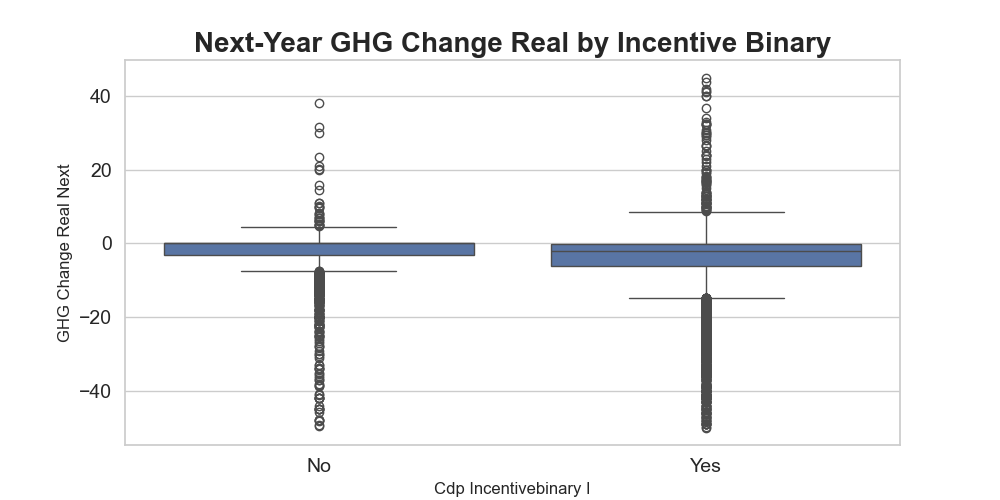
\includegraphics[width=\textwidth]{figures/ghg_change_real_next_by_cdp_incentivebinary_i.png}
\caption{Incentive Binary vs. Next Year Decarbonization Rate}
\label{fig:ghg_change_real_next_by_cdp_incentivebinary_i}
\end{figure}

\begin{figure}[H]
    % ghg_change_real_next_by_method_ind
\centering
    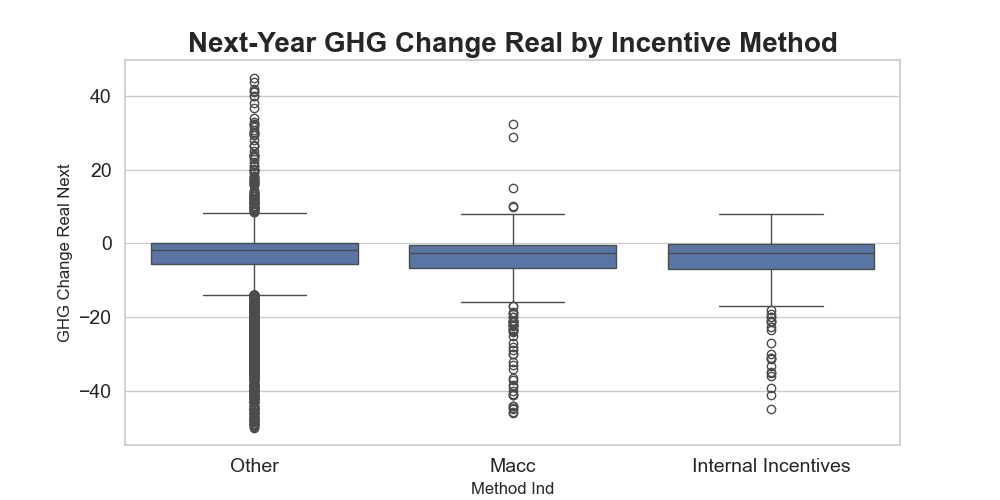
\includegraphics[width=\textwidth]{figures/ghg_change_real_next_by_method_ind.png}
\caption{Incentive Method vs. Next Year Decarbonization Rate}
\label{fig:ghg_change_real_next_by_method_ind}
\end{figure}

\subsection{Discussion on Incentives}

\begin{itemize}
    \item The analysis from the first model indicates that simply having incentives in place (Cdp.Incentivebinary.I) is significantly associated with a decarbonization rate, with a negative coefficient (-0.561, significant at the 1\% level). The marginal relationship can be observed in Figure \ref{fig:ghg_change_real_next_by_cdp_incentivebinary_i}. This suggests that firms with any form of incentives aimed at reducing emissions are correlated with relatively better decarbonization efforts compared to those without as expected.

    \item When analyzing the types of incentives in the second model, we observe how specific incentive methods have better outcomes than general incentives. In particular, the Method.IndInternal Incentives (internal incentives for decarbonization) show a very strong negative relationship with the decarbonization rate (-1.776, significant at the 1\% level), indicating that internal corporate incentives are particularly effective compare to the "other" baseline. Similarly, Method.IndMacc (Marginal Abatement Cost Curve) also show a negative coefficient (-0.807, significant at the 5\% level), suggesting that firms who use a marginal abatement cost curve to reward decarbonization efforts are correlated with a better decarboninzation performance. For more details on the Marginal Abatement Cost Curve, see Appendix \ref{sec:MACC}. Additionally, the marginal relationship between inective methods and next-year decarbonization rates is presented in Figure \ref{fig:ghg_change_real_next_by_method_ind} wehre we observe how internal incetives and using the Marginal Abatement Cost Curve are both correlated with better average decarbonization rates compared to other forms of incentives.


    \item The consistent negative coefficients for incentives across models demonstrate that well-structured incentive programs, especially those embedded within the company's internal operations, can be useufl  for achieving meaningful decarbonization not only on a same year basis, but also when considering next-year decarbonizaiton rate. This could imply that incentives not only drive immediate actions but also foster a culture of sustainability and long-term commitment to reducing emissions.

    \item Interestingly, board oversight did not emerge as a significant factor in the final model, suggesting that while governance is important, the direct impact on decarbonization rates may be more strongly influenced by tangible, operational incentive mechanisms rather than solely by high-level oversight.
    \item \textbf{Key Findings:} Our study highlights the significant role of targeted incentives in enhancing a firm's decarbonization efforts. Specifically, internal incentives and the use of Marginal Abatement Cost Curves are notably effective. This suggests that detailed, well-implemented incentive schemes are key to reducing emissions, more so than general executive endorsements or board oversight.

\end{itemize}


\section{Model VII: Analyzing Targets, Risks, and Opportunities}

\begin{enumerate}
    \item First model: we analyze the role that targets play in forecasting next-year decarbonization. In particular, we look at both absolute figures (such as target amount) and target types

    \item Second model: This model adds in how companies perceive their environmental risks and opportunities. It checks if recognizing more risks or seeing more green opportunities changes how well they can reduce emissions, alongside their financial metrics and targets.
    \item Third model: third model combines all predictors from targets, risk, and opportunities together.
    \item Fourth model: The final model narrows down excluding variables that are not significant at the 5\% level
\end{enumerate}


\begin{table}[H] \centering    \caption{Impact of GHG, Verification, Incentives, Targets, Risks and Opportunities on Decarbonization}    \label{tab:R7}  \resizebox{0.8\textwidth}{!}{\begin{tabular}{@{\extracolsep{5pt}}lcccc}  \\[-1.8ex]\hline  \hline \\[-1.8ex]   & \multicolumn{4}{c}{\textit{Dependent variable:}} \\  \cline{2-5}  \\[-1.8ex] & \multicolumn{4}{c}{Next Year Decarbonization Rate} \\  \\[-1.8ex] & (1) & (2) & (3) & (4)\\  \hline \\[-1.8ex]   Year & $-$0.087$^{***}$ (0.028) & $-$0.057$^{*}$ (0.031) & $-$0.040 (0.031) & $-$0.047 (0.031) \\    Ghg.Change.Real & 0.191$^{***}$ (0.009) & 0.192$^{***}$ (0.009) & 0.188$^{***}$ (0.009) & 0.188$^{***}$ (0.009) \\    Market.Cap & $-$0.403$^{***}$ (0.084) & $-$0.400$^{***}$ (0.086) & $-$0.410$^{***}$ (0.085) & $-$0.409$^{***}$ (0.085) \\    Revenue & 0.241$^{**}$ (0.094) & 0.187$^{**}$ (0.095) & 0.247$^{***}$ (0.094) & 0.249$^{***}$ (0.094) \\    Type.Scope1Limited/Moderate & 0.344 (0.220) & 0.347 (0.222) & 0.369$^{*}$ (0.220) & 0.370$^{*}$ (0.220) \\    Type.Scope1N.A & 0.746$^{***}$ (0.263) & 0.867$^{***}$ (0.264) & 0.769$^{***}$ (0.263) & 0.796$^{***}$ (0.262) \\    Type.Scope1Third.Party.Underway & 0.738$^{**}$ (0.294) & 0.809$^{***}$ (0.296) & 0.774$^{***}$ (0.295) & 0.792$^{***}$ (0.294) \\    Ghg.Verification.Scope3.Yes & $-$0.325$^{*}$ (0.181) & $-$0.401$^{**}$ (0.181) & $-$0.309$^{*}$ (0.181) & $-$0.317$^{*}$ (0.181) \\    Ghg1 & 0.123$^{***}$ (0.034) & 0.121$^{***}$ (0.035) & 0.122$^{***}$ (0.035) & 0.122$^{***}$ (0.034) \\    Ghg2Location & $-$0.059$^{**}$ (0.025) & $-$0.054$^{**}$ (0.025) & $-$0.052$^{**}$ (0.025) & $-$0.052$^{**}$ (0.025) \\    Ghg3.Count & $-$0.033 (0.025) & $-$0.060$^{**}$ (0.024) & $-$0.031 (0.025) & $-$0.032 (0.024) \\    Ghg1.Na & 1.673$^{***}$ (0.503) & 1.676$^{***}$ (0.507) & 1.637$^{***}$ (0.503) & 1.657$^{***}$ (0.502) \\    Ghg2Market.Na & 0.897$^{***}$ (0.178) & 1.005$^{***}$ (0.178) & 0.915$^{***}$ (0.178) & 0.911$^{***}$ (0.178) \\    Methane.Emissions & 0.078$^{***}$ (0.022) & 0.082$^{***}$ (0.022) & 0.081$^{***}$ (0.022) & 0.083$^{***}$ (0.022) \\    Method.IndInternal Incentives & $-$1.681$^{***}$ (0.572) & $-$1.740$^{***}$ (0.576) & $-$1.678$^{***}$ (0.572) & $-$1.700$^{***}$ (0.572) \\    Method.IndMacc & $-$0.775$^{**}$ (0.364) & $-$0.736$^{**}$ (0.367) & $-$0.723$^{**}$ (0.364) & $-$0.725$^{**}$ (0.364) \\    Cdp.Incentivebinary.I & $-$0.356$^{*}$ (0.192) & $-$0.491$^{**}$ (0.193) & $-$0.300 (0.195) &  \\    Cdp.Baseyearemission.Mean & 0.016 (0.016) &  & 0.016 (0.016) &  \\    Cdp.Targetscope.Percent.Mean & 0.001 (0.002) &  & 0.001 (0.002) &  \\    Cdp.Targetamount.Mean & $-$0.433$^{***}$ (0.073) &  & $-$0.420$^{***}$ (0.073) & $-$0.368$^{***}$ (0.054) \\    Cdp.Targettype.Absolute & $-$0.194$^{***}$ (0.066) &  & $-$0.181$^{***}$ (0.066) & $-$0.165$^{***}$ (0.058) \\    Cdp.Targettype.Intensity & 0.088 (0.069) &  & 0.086 (0.069) &  \\    Cdp.Aggregated.Risk &  & 0.615$^{***}$ (0.178) & 0.565$^{***}$ (0.177) & 0.553$^{***}$ (0.176) \\    Cdp.Aggregated.Opp &  & $-$1.283$^{***}$ (0.238) & $-$1.151$^{***}$ (0.237) & $-$1.184$^{***}$ (0.236) \\    Constant & 0.193 (1.512) & 1.110 (1.543) & 0.362 (1.534) & 0.232 (1.525) \\   \hline \\[-1.8ex]  \textbf{Random Effects:} &  &  &  &  \\  Number of Firms & 1871 & 1871 & 1871 & 1871 \\  Number of Industries & 25 & 25 & 25 & 25 \\  Number of Continents & 6 & 6 & 6 & 6 \\  Number of Countries & 48 & 48 & 48 & 48 \\  sd(Firms:Industry) & 1.47 & 1.58 & 1.495 & 1.49 \\  sd(Industry) & 0.588 & 0.653 & 0.593 & 0.605 \\  sd(Continent) & 0.614 & 0.651 & 0.619 & 0.617 \\  sd(Country:Continent) & 0.219 & 0.197 & 0.218 & 0.219 \\  Akaike Inf. Crit. & 93634.714 & 93641.746 & 93614.903 & 93589.986 \\  Bayesian Inf. Crit. & 93845.502 & 93829.949 & 93840.747 & 93785.717 \\  \hline  \hline \\[-1.8ex]  \textit{Note:}  & \multicolumn{4}{r}{$^{*}$p$<$0.1; $^{**}$p$<$0.05; $^{***}$p$<$0.01} \\   & \multicolumn{4}{r}{Sixth Model focuses on GHG, Verification, and Incentives} \\  \end{tabular}}  \end{table} 

\subsection{Relevant Figures:}

% first figure cdp_target_amount_vs_ghg_change_real_next
\begin{figure}[H]
\centering
  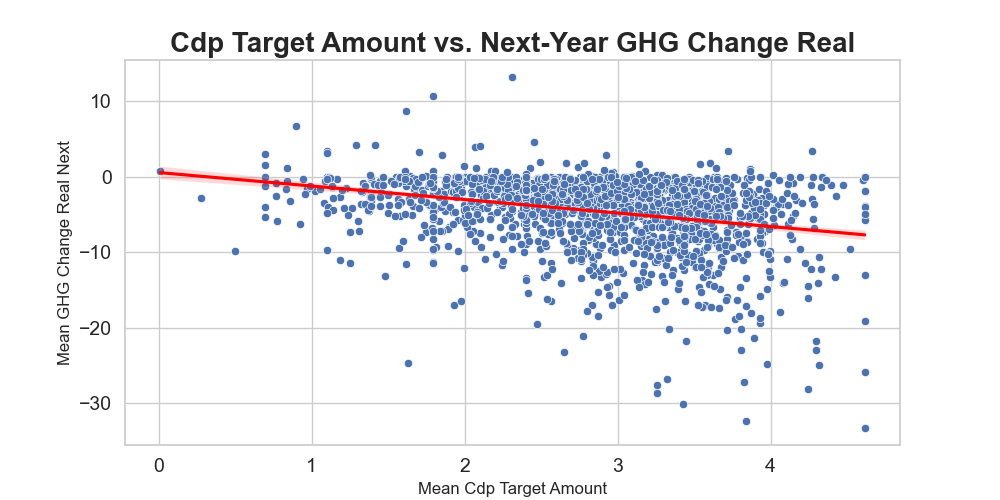
\includegraphics[width=\textwidth]{figures/cdp_target_amount_vs_ghg_change_real_next.png}
\caption{Cdp Target Amount vs. Next Year Decarbonization Rate}
\label{fig:cdp_target_amount_vs_ghg_change_real_next}
\end{figure}

% second figure cdp_target_type_absolute_vs_ghg_change_real_next
\begin{figure}[H]
\centering
  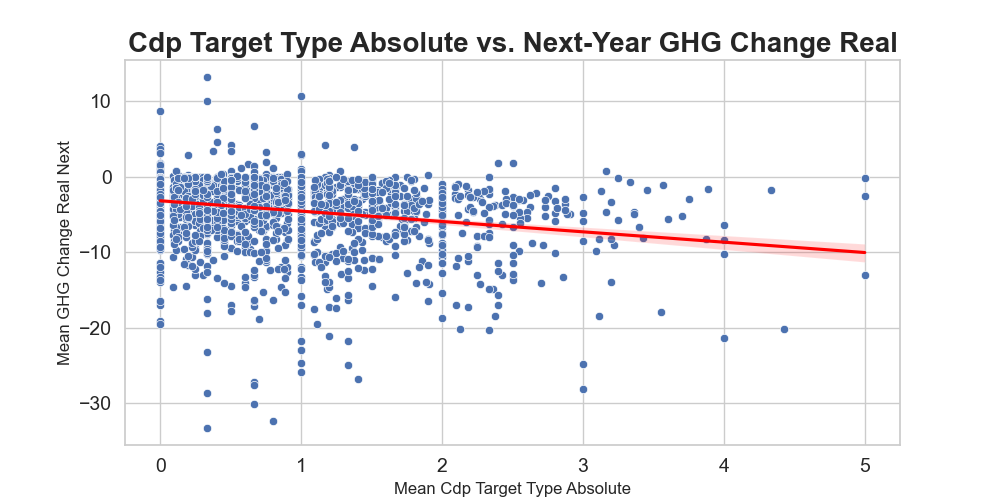
\includegraphics[width=\textwidth]{figures/cdp_target_type_absolute_vs_ghg_change_real_next.png}
\caption{Cdp Target Type Absolute vs. Next Year Decarbonization Rate}
\label{fig:cdp_target_type_absolute_vs_ghg_change_real_next}
\end{figure}

% third figure ghg_change_real_next_by_cdp_aggregated_risk
\begin{figure}[H]
\centering
  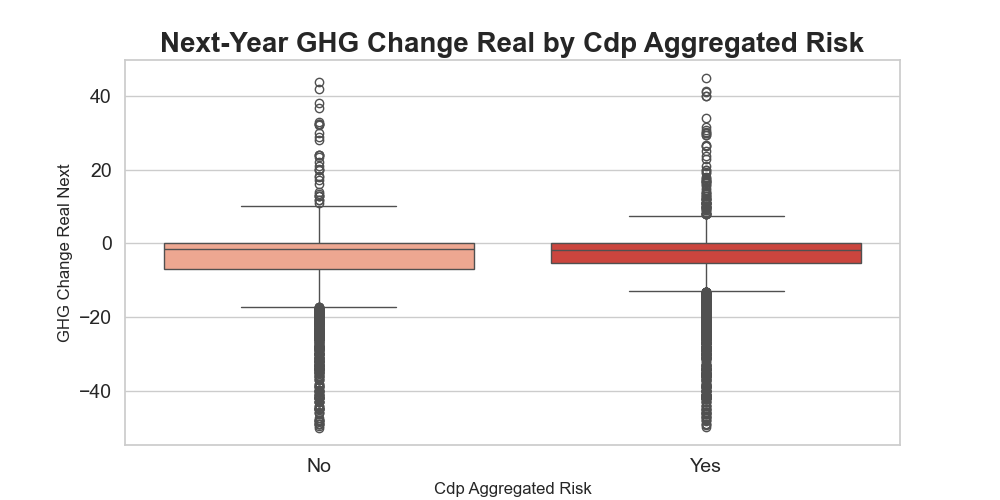
\includegraphics[width=\textwidth]{figures/ghg_change_real_next_by_cdp_aggregated_risk.png}
\caption{Cdp Aggregated Risk vs. Next Year Decarbonization Rate}
\label{fig:ghg_change_real_next_by_cdp_aggregated_risk}
\end{figure}

% fourth figure ghg_change_real_next_by_cdp_aggregated_opportunity
\begin{figure}[H]
\centering
  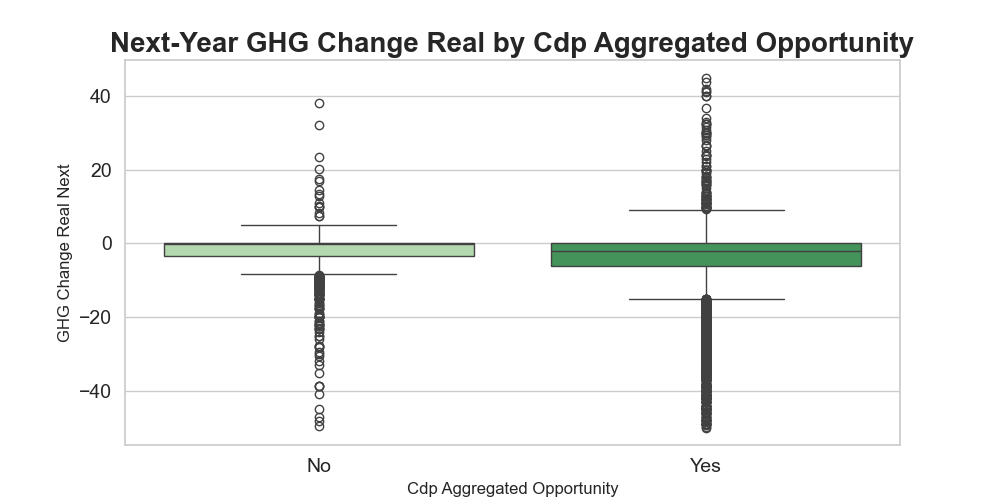
\includegraphics[width=\textwidth]{figures/ghg_change_real_next_by_cdp_aggregated_opportunity.png}
\caption{Cdp Aggregated Opportunity vs. Next Year Decarbonization Rate}
\label{fig:ghg_change_real_next_by_cdp_aggregated_opportunity}
\end{figure}


\subsection{Discussion}
\begin{itemize}
\item The results suggest that setting specific emission reduction targets (Cdp.Targetamount.Mean) has a significant negative impact on the next year's decarbonization rate, with coefficients like $-0.433$ (significant at the 1\% level). This indicates that firms with more ambitious targets are correlated with a better decarboninzation rate. This can also be seen in the Figure \ref{fig:cdp_target_amount_vs_ghg_change_real_next}, where we observe a negative relationship between the target amount and the decarbonization rate. This suggests that firms with higher target amounts are expected to have a better next-year decarbonization rate. 
\item The type of target set by firms also matters. Companies with absolute reduction targets (Cdp.Targettype.Absolute) show a notable improvement in decarbonization efforts, as indicated by a negative coefficient of -0.194 (significant at the 1\% level) this relationship is also showin in Figure \ref{fig:cdp_target_type_absolute_vs_ghg_change_real_next} where we observe a slight negative trend between absolute targets and decarbonization rate. This contrasts with intensity-based targets (Cdp.Targettype.Intensity), which did not show significant effects, suggesting that absolute targets might be more impactful.

\item Assessing risks (Cdp.Aggregated.Risk) and identifying opportunities (Cdp.Aggregated.Opp) associated with climate change also appear to influence decarbonization rates significantly. Firms recognizing risks show a negative impact on decarbonization rate with a coefficient of 0.615 (significant at the 1\% level), indicating that firms that identify risks are correlated with lower decarboninzation, this relationship can also be observed in the boxplot in Figure \ref{fig:ghg_change_real_next_by_cdp_aggregated_risk} where we observe a positive relationship between the aggregated risk and the decarbonization rate. Conversely, recognizing opportunities related to climate change is linked with better decarbonization outcomes, as shown by a negative coefficient of -1.283 (significant at the 1\% level), suggesting that firms identifying decarboninzation opportunities tend to reduce their emissions over the next year. The relationship between opportunities and next year real decarbonization rate is also shown in Figure \ref{fig:ghg_change_real_next_by_cdp_aggregated_opportunity} where we observe that the distribution of firms who identify an opportunity corresponds to a relatively lower next-year decarbonization rate.

\item \textbf{Key findings:} Targets play an important role in enhancing decarbonization rates over the next year, and an understanding of risks and opportunities, is equally important. Additionally, to gain a comprehensive understanding, it is most valuable to observe the mean amount target set by a firm, and whether that firm has identified risks and opportunites.

\end{itemize}

\section{Model VIII: Analyzing Investments and Initiatives}

\begin{enumerate}
    \item First model: We analyze the predictors related to initiatives, in particual whether the company has initiatives to reduce carbon emissions and which scopes have a related initiative. 
    \item Second model: we analyze investments that companies make to reduce carbon emissions by looking at the number of invesmtents, the potential GHG savings, and the estimated capital requirement to execute the investments.
    \item Third model: we combine all predicors together to then perform feature selection.
    \item Fourth model: The final model revomes non-significant predcitors to enhance the AIC score and strike an optimal balance between number of features and forecasting ability.
\end{enumerate}


\begin{table}[H] \centering    \caption{Impact of GHG, Verification, Incentives, Targets, Risks and Opportunities, Initiatives, Investments on Decarbonization}    \label{tab:R8}  \resizebox{0.7\textwidth}{!}{\begin{tabular}{@{\extracolsep{5pt}}lcccc}  \\[-1.8ex]\hline  \hline \\[-1.8ex]   & \multicolumn{4}{c}{\textit{Dependent variable:}} \\  \cline{2-5}  \\[-1.8ex] & \multicolumn{4}{c}{Next Year Decarbonization Rate} \\  \\[-1.8ex] & (1) & (2) & (3) & (4)\\  \hline \\[-1.8ex]   Year & $-$0.049 (0.034) & $-$0.038 (0.031) & $-$0.059$^{*}$ (0.034) & $-$0.068$^{**}$ (0.032) \\    Ghg.Change.Real & 0.188$^{***}$ (0.009) & 0.186$^{***}$ (0.009) & 0.185$^{***}$ (0.009) & 0.186$^{***}$ (0.009) \\    Market.Cap & $-$0.406$^{***}$ (0.085) & $-$0.397$^{***}$ (0.084) & $-$0.400$^{***}$ (0.085) & $-$0.403$^{***}$ (0.084) \\    Revenue & 0.270$^{***}$ (0.094) & 0.252$^{***}$ (0.094) & 0.269$^{***}$ (0.094) & 0.268$^{***}$ (0.094) \\    Type.Scope1Limited/Moderate & 0.388$^{*}$ (0.220) & 0.352 (0.220) & 0.373$^{*}$ (0.220) & 0.370$^{*}$ (0.220) \\    Type.Scope1N.A & 0.771$^{***}$ (0.261) & 0.728$^{***}$ (0.262) & 0.730$^{***}$ (0.262) & 0.723$^{***}$ (0.262) \\    Type.Scope1Third.Party.Underway & 0.770$^{***}$ (0.294) & 0.717$^{**}$ (0.295) & 0.731$^{**}$ (0.295) & 0.724$^{**}$ (0.294) \\    Ghg.Verification.Scope3.Yes & $-$0.307$^{*}$ (0.180) & $-$0.261 (0.181) & $-$0.264 (0.181) & $-$0.261 (0.181) \\    Ghg1 & 0.109$^{***}$ (0.035) & 0.123$^{***}$ (0.034) & 0.108$^{***}$ (0.035) & 0.112$^{***}$ (0.035) \\    Ghg2Location & $-$0.048$^{*}$ (0.025) & $-$0.047$^{*}$ (0.025) & $-$0.045$^{*}$ (0.025) & $-$0.045$^{*}$ (0.025) \\    Ghg3.Count & $-$0.027 (0.025) & $-$0.013 (0.025) & $-$0.014 (0.025) & $-$0.012 (0.025) \\    Ghg1.Na & 1.437$^{***}$ (0.507) & 1.668$^{***}$ (0.502) & 1.423$^{***}$ (0.508) & 1.465$^{***}$ (0.506) \\    Ghg2Market.Na & 0.888$^{***}$ (0.179) & 0.913$^{***}$ (0.178) & 0.904$^{***}$ (0.179) & 0.916$^{***}$ (0.178) \\    Methane.Emissions & 0.079$^{***}$ (0.022) & 0.083$^{***}$ (0.022) & 0.080$^{***}$ (0.022) & 0.081$^{***}$ (0.022) \\    Method.IndInternal Incentives & $-$1.667$^{***}$ (0.571) & $-$1.752$^{***}$ (0.571) & $-$1.714$^{***}$ (0.571) & $-$1.705$^{***}$ (0.571) \\    Method.IndMacc & $-$0.710$^{*}$ (0.364) & $-$0.716$^{**}$ (0.363) & $-$0.704$^{*}$ (0.363) & $-$0.705$^{*}$ (0.363) \\    Cdp.Targetamount.Mean & $-$0.349$^{***}$ (0.055) & $-$0.345$^{***}$ (0.055) & $-$0.335$^{***}$ (0.055) & $-$0.332$^{***}$ (0.055) \\    Cdp.Targettype.Absolute & $-$0.164$^{***}$ (0.058) & $-$0.153$^{***}$ (0.058) & $-$0.156$^{***}$ (0.058) & $-$0.160$^{***}$ (0.058) \\    Cdp.Aggregated.Risk & 0.584$^{***}$ (0.180) & 0.617$^{***}$ (0.178) & 0.584$^{***}$ (0.181) & 0.574$^{***}$ (0.178) \\    Cdp.Aggregated.Opp & $-$1.109$^{***}$ (0.237) & $-$1.132$^{***}$ (0.236) & $-$1.073$^{***}$ (0.237) & $-$1.063$^{***}$ (0.237) \\    Initiative.Scope1 & 0.258$^{**}$ (0.124) &  & 0.311$^{**}$ (0.125) & 0.275$^{**}$ (0.117) \\    Initiative.Scope2 & $-$0.153 (0.113) &  & $-$0.072 (0.115) &  \\    Initiative.Scope3 & $-$0.149 (0.165) &  & $-$0.040 (0.170) &  \\    Absent.Cdp.Initiative.Firm.Year.Processed.Csv & 0.855$^{***}$ (0.269) &  & 0.725$^{**}$ (0.283) & 0.752$^{***}$ (0.269) \\    Co2.Counter &  & $-$0.135 (0.084) & $-$0.106 (0.088) &  \\    Msaving.Counter &  & 0.183$^{*}$ (0.105) & 0.177$^{*}$ (0.105) &  \\    Investment.Counter &  & $-$0.313$^{***}$ (0.121) & $-$0.358$^{***}$ (0.122) & $-$0.278$^{***}$ (0.064) \\    Investment.Total.Log1P &  & $-$0.002 (0.015) & 0.007 (0.015) &  \\    Constant & $-$0.364 (1.531) & $-$0.072 (1.522) & $-$0.368 (1.529) & $-$0.345 (1.532) \\   \hline \\[-1.8ex]  \textbf{Random Effects:} &  &  &  &  \\  Number of Firms & 1871 & 1871 & 1871 & 1871 \\  Number of Industries & 25 & 25 & 25 & 25 \\  Number of Continents & 6 & 6 & 6 & 6 \\  Number of Countries & 48 & 48 & 48 & 48 \\  sd(Firms:Industry) & 1.474 & 1.467 & 1.461 & 1.468 \\  sd(Industry) & 0.584 & 0.608 & 0.59 & 0.593 \\  sd(Continent) & 0.631 & 0.612 & 0.63 & 0.639 \\  sd(Country:Continent) & 0.207 & 0.2 & 0.2 & 0.231 \\  Akaike Inf. Crit. & 93589.449 & 93590.17 & 93593.274 & 93570.684 \\  Bayesian Inf. Crit. & 93815.293 & 93816.014 & 93849.23 & 93789 \\  \hline  \hline \\[-1.8ex]  \textit{Note:}  & \multicolumn{4}{r}{$^{*}$p$<$0.1; $^{**}$p$<$0.05; $^{***}$p$<$0.01} \\   & \multicolumn{4}{r}{Seventh Model focuses on GHG, Verification, and Incentives} \\  \end{tabular}}  \end{table} 

\subsection{Relevant Figures:}

% first figure ghg_change_real_next_by_absent_cdp_initiative
\begin{figure}[H]
\centering
  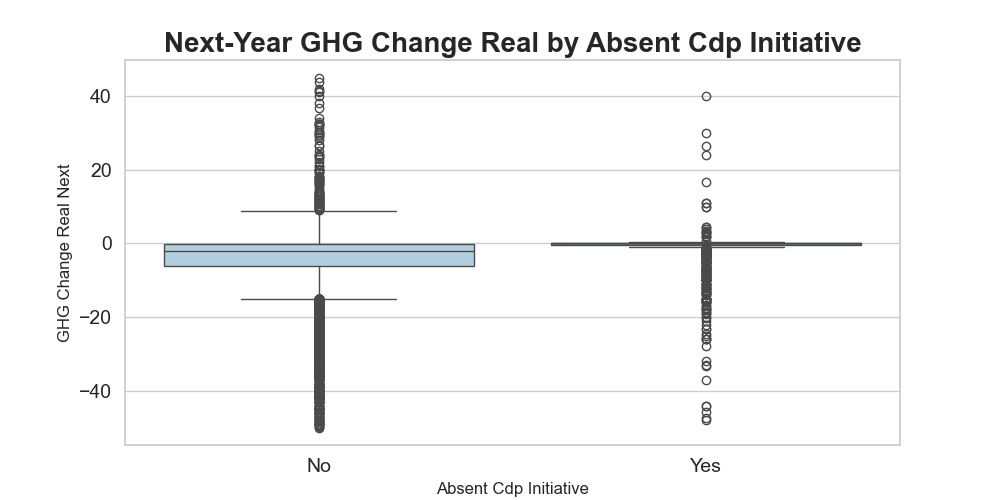
\includegraphics[width=\textwidth]{figures/ghg_change_real_next_by_absent_cdp_initiative.png}
\caption{Absent Cdp Initiative vs. Next Year Decarbonization Rate}
\label{fig:ghg_change_real_next_by_absent_cdp_initiative}
\end{figure}

% second figure ghg_change_real_next_by_investment_counter
\begin{figure}[H]
\centering
  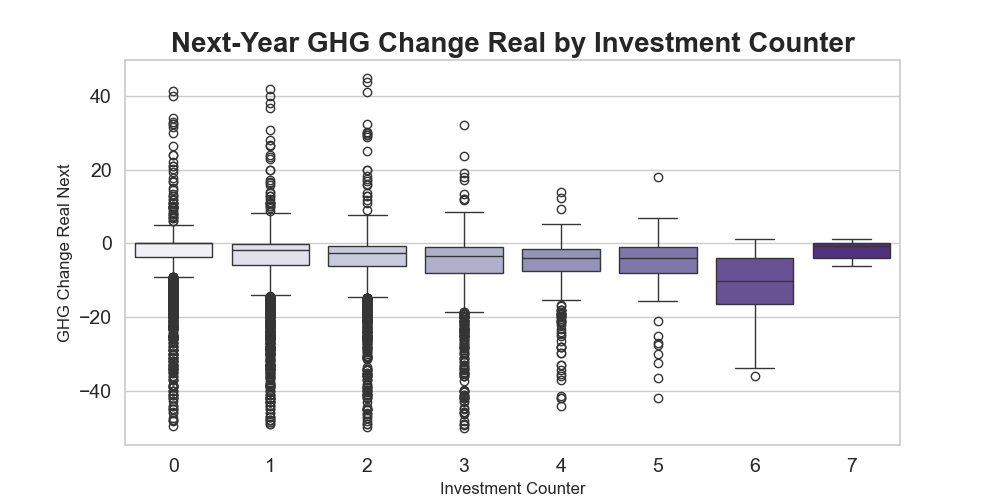
\includegraphics[width=\textwidth]{figures/ghg_change_real_next_by_investment_counter.png}
\caption{Investment Counter vs. Next Year Decarbonization Rate}
\label{fig:ghg_change_real_next_by_investment_counter}
\end{figure}




\subsection{Discussion}

\begin{itemize}
    \item The only significant initiative metrics are whether the company does not have any initiatives, associated with a worse decarboninzation of $0.855$, and whether the company has initiatives on scope $1$, which is associated with worse decarbonization rate of $0.258\%$. The relationship between the absence of initiatives and next year decarbonization rate is also shown in Figure \ref{fig:ghg_change_real_next_by_absent_cdp_initiative}, where we observe that firms who don't report initiatives also have a decarbonization rate of zero, that is either they don't decarbonize, or they don't accurately report their decarbonization efforts. The Scope 1 coefficient makes sense given the context of the model as it likely acts as an indicator of whether a firm that has incentives has them in Scope 1 emissions or in either Scope 2 or Scope 3. With having incentives in Scope 2/3 being associated with better decarboninzation rates. 
    \item The absolute number of investments is significant and associated with a better decarboninzation rate of $2.78\%$ per investment in model (4). Other invesmtent metrics are not significant at the $5\%$ level and were not included in the final model. The relationship between the number of investments and the next year decarbonization rate is also shown in Figure \ref{fig:ghg_change_real_next_by_investment_counter}.
    \item \textbf{Key Insights:} Investments and Initiatives are important components of carbon emission reduction. Based on this analysis, which is correlational, they have an effect on decarboninzation that goes past the same year and affects the following year as well. This makes intutitive sense as we expect the investment that a firm makes along with economic incentives to have an effect over time as in both cases positive outcomes result in systemic change has a positive impact over time.
\end{itemize}

\section{Model IX: Analyzing Carbon Credits and Intensity Figures}

\begin{enumerate}
    \item First model: We analyze the predictors related to intensity figures and intensity change controlling for all other variables carried forward from previous models.
    \item Second Model: similar to model (1), but we perform inference on the same-year by using as response Ghg.Change.Real and controlling for Ghg.Change.Real.Prev (lag-1 variable of Ghg.Change.Real)
    \item Third model: we analyze carbon credits and the impact that they have on next year decarboninzation rate, still controlling for all other variable carried forward from previous models.
\end{enumerate}

\begin{table}[H] \centering    \caption{Impact of Carbon Credits and Intensity Figures on Next-Year Real Decarbonization Rate}    \label{tab:R9}  \resizebox{0.7\textwidth}{!}{\begin{tabular}{@{\extracolsep{5pt}}lccc}  \\[-1.8ex]\hline  \hline \\[-1.8ex]   & \multicolumn{3}{c}{\textit{Dependent variable:}} \\  \cline{2-4}  \\[-1.8ex] & Ghg.Change.Real.Next & Ghg.Change.Real & Ghg.Change.Real.Next \\  \\[-1.8ex] & (26) & (27) & (28)\\  \hline \\[-1.8ex]   Ghg.Change.Real & 0.187$^{***}$ (0.009) &  & 0.186$^{***}$ (0.009) \\    Ghg.Change.Real.Prev &  & 0.114$^{***}$ (0.008) &  \\    Year & $-$0.038 (0.031) & 0.016 (0.029) & $-$0.045 (0.031) \\    Market.Cap & $-$0.396$^{***}$ (0.084) & $-$0.204$^{**}$ (0.080) & $-$0.396$^{***}$ (0.085) \\    Revenue & 0.260$^{***}$ (0.094) & 0.177$^{**}$ (0.088) & 0.262$^{***}$ (0.094) \\    Type.Scope1Limited/Moderate & 0.362$^{*}$ (0.220) & 0.258 (0.207) & 0.347 (0.220) \\    Type.Scope1N.A & 0.730$^{***}$ (0.262) & 0.491$^{**}$ (0.246) & 0.702$^{***}$ (0.262) \\    Type.Scope1Third.Party.Underway & 0.730$^{**}$ (0.295) & 0.527$^{*}$ (0.275) & 0.696$^{**}$ (0.294) \\    Ghg.Verification.Scope3.Yes & $-$0.259 (0.181) & $-$0.569$^{***}$ (0.169) & $-$0.252 (0.181) \\    Ghg1 & 0.124$^{***}$ (0.034) & 0.149$^{***}$ (0.031) & 0.125$^{***}$ (0.034) \\    Ghg2Location & $-$0.049$^{**}$ (0.025) & $-$0.017 (0.023) & $-$0.046$^{*}$ (0.025) \\    Ghg3.Count & $-$0.012 (0.025) & $-$0.067$^{***}$ (0.023) & $-$0.010 (0.025) \\    Ghg1.Na & 1.633$^{***}$ (0.503) & 1.512$^{***}$ (0.462) & 1.612$^{***}$ (0.502) \\    Ghg2Market.Na & 0.912$^{***}$ (0.178) & 0.951$^{***}$ (0.165) & 0.904$^{***}$ (0.178) \\    Methane.Emissions & 0.082$^{***}$ (0.022) & 0.029 (0.020) & 0.082$^{***}$ (0.022) \\    Method.IndInternal Incentives & $-$1.722$^{***}$ (0.571) & $-$0.560 (0.534) & $-$1.710$^{***}$ (0.571) \\    Method.IndMacc & $-$0.707$^{*}$ (0.363) & $-$0.744$^{**}$ (0.342) & $-$0.698$^{*}$ (0.363) \\    Cdp.Targetamount.Mean & $-$0.340$^{***}$ (0.055) & $-$0.455$^{***}$ (0.051) & $-$0.330$^{***}$ (0.055) \\    Cdp.Targettype.Absolute & $-$0.153$^{***}$ (0.058) & $-$0.122$^{**}$ (0.055) & $-$0.152$^{***}$ (0.058) \\    Cdp.Aggregated.Risk & 0.623$^{***}$ (0.177) & 0.472$^{***}$ (0.163) & 0.623$^{***}$ (0.177) \\    Cdp.Aggregated.Opp & $-$1.098$^{***}$ (0.237) & $-$0.796$^{***}$ (0.220) & $-$1.081$^{***}$ (0.237) \\    Absent.Cdp.Initiative.Firm.Year.Processed.Csv & 0.733$^{***}$ (0.270) & 0.574$^{**}$ (0.250) & 0.678$^{**}$ (0.267) \\    Investment.Counter & $-$0.254$^{***}$ (0.063) & $-$0.377$^{***}$ (0.058) & $-$0.247$^{***}$ (0.062) \\    Ghg.Int.Figure.Na & $-$2.861 (1.888) & $-$0.402 (1.739) &  \\    Ghg.Int.Figure & 0.021 (0.034) & 0.028 (0.031) &  \\    Ghg.Int.Change & $-$0.001 (0.003) & 0.059$^{***}$ (0.003) &  \\    Absent.Cdp.Ghg.Int.Processed.Csv & $-$0.266 (0.201) & 0.069 (0.186) &  \\    Cdp.Num.Credits.Clean.Count &  &  & 0.011 (0.043) \\    Cdp.Orig.Or.Purchase.Clean.Credit.Origination &  &  & 0.006 (0.062) \\    Cdp.Purpose.Clean.Voluntary.Offsetting &  &  & $-$0.048 (0.067) \\    Absent.Cdp.Carbon.Credits.Full.Processed.Csv &  &  & 0.067 (0.196) \\    Constant & $-$0.423 (1.533) & $-$2.738$^{*}$ (1.459) & $-$0.578 (1.559) \\   \hline \\[-1.8ex]  \textbf{Random Effects:} &  &  &  \\  Number of Firms & 1871 & 1871 & 1871 \\  Number of Industries & 25 & 25 & 25 \\  Number of Continents & 6 & 6 & 6 \\  Number of Countries & 48 & 48 & 48 \\  sd(Firms:Industry) & 1.466 & 1.604 & 1.468 \\  sd(Industry) & 0.605 & 0.425 & 0.602 \\  sd(Continent) & 0.625 & 0.53 & 0.625 \\  sd(Country:Continent) & 0.213 & 0.446 & 0.227 \\  Akaike Inf. Crit. & 93587.623 & 91292.459 & 93593.136 \\  Bayesian Inf. Crit. & 93828.524 & 91533.357 & 91533.357 \\  \hline  \hline \\[-1.8ex]  \textit{Note:}  & \multicolumn{3}{r}{$^{*}$p$<$0.1; $^{**}$p$<$0.05; $^{***}$p$<$0.01} \\ \multicolumn{4}{p{1.5\textwidth}}{\textit{Model (26): We analyze the predictors related to intensity figures and intensity change controlling for all other variables carried forward from previous models. Model (27): similar to model (26), but we perform inference on the same-year by using as response Ghg.Change.Real and controlling for Ghg.Change.Real.Prev (lag-1 variable of Ghg.Change.Real). Model (28): we analyze carbon credits and the impact that they have on next year decarboninzation rate, still controlling for all other variable carried forward from previous models.}} \\  \end{tabular}}  \end{table}

\subsection{Discussion}

\begin{itemize}
    \item Intensity is a variable that is important when assessing decarbonization and in model (2) intensity change is significant and positive as expected. Though, in model (1) the predictor is not significant and the coefficient value is almost $0$, this seems to suggest that while intensity can explain same-year emissions, given the other control varaibles present in the model, it has little predictive power on next year emisssions.
    \item Carbon Credits show no rpedictive power for next year emissions, this makes sense as carbon credits have no impact on \textit{Real} Decarbonization Rate which can be achieved only through utilization of a greater share of renewable energy or by enhacning internal processes.
    \item \textbf{Key Insights: } Neither Intensity figures nor Carbon Credits are useufl predictors when assessing next year real decarbonization rate. Therefore, I will exculde them from the final model.
\end{itemize}

\section{Model X: Final Models}


\begin{enumerate}
    \item First model: result of applying backward stepwise regression to eliminate non-significant control variables and random effects to generate a final model with the best AIC
    \item Second model: adding back some predicors that I believe are important and that were analyse before, the model is very similar to model (1), with the only difference that we don't remove the coefficient for year and the random intercept for country.
    \item Third model: testing model (2) on same-year decarboninzation rate controlling for Ghg.Change.Real.Lag1 to check which predictors are significant in predicting same-year decarboninzation rates and pefrom a final comparison
\end{enumerate}

\begin{table}[H] \centering    \caption{Impact of Selected Predictors on Next-Year Real Decarbonization Rate}    \label{tab:R10}  \resizebox{0.8\textwidth}{!}{\begin{tabular}{@{\extracolsep{5pt}}lccc}  \\[-1.8ex]\hline  \hline \\[-1.8ex]   & \multicolumn{3}{c}{\textit{Dependent variable:}} \\  \cline{2-4}  \\[-1.8ex] & \multicolumn{2}{c}{Next Year Decarbonization Rate} & Ghg.Change.Real \\  \\[-1.8ex] & (1) & (2) & (3)\\  \hline \\[-1.8ex]   Year &  & $-$0.048 (0.030) & $-$0.013 (0.028) \\    Ghg.Change.Real & 0.188$^{***}$ (0.009) & 0.186$^{***}$ (0.009) &  \\    Ghg.Change.Real.Lag1 &  &  & 0.117$^{***}$ (0.008) \\    Market.Cap & $-$0.414$^{***}$ (0.084) & $-$0.398$^{***}$ (0.084) & $-$0.253$^{***}$ (0.080) \\    Revenue & 0.245$^{***}$ (0.091) & 0.257$^{***}$ (0.094) & 0.163$^{*}$ (0.089) \\    Type.Scope1Limited/Moderate & 0.361$^{*}$ (0.218) & 0.358 (0.220) & 0.235 (0.209) \\    Type.Scope1N.A & 0.914$^{***}$ (0.242) & 0.720$^{***}$ (0.261) & 0.534$^{**}$ (0.249) \\    Type.Scope1Third.Party.Underway & 0.833$^{***}$ (0.291) & 0.713$^{**}$ (0.294) & 0.535$^{*}$ (0.277) \\    Ghg.Verification.Scope3.Yes &  & $-$0.272 (0.178) & $-$0.667$^{***}$ (0.169) \\    Ghg1 & 0.115$^{***}$ (0.033) & 0.125$^{***}$ (0.034) & 0.179$^{***}$ (0.032) \\    Ghg2Location &  & $-$0.046$^{*}$ (0.025) & $-$0.022 (0.023) \\    Ghg1.Na & 1.954$^{***}$ (0.472) & 1.614$^{***}$ (0.502) & 1.845$^{***}$ (0.466) \\    Ghg2Market.Na & 1.026$^{***}$ (0.149) & 0.917$^{***}$ (0.177) & 1.030$^{***}$ (0.166) \\    Methane.Emissions & 0.075$^{***}$ (0.022) & 0.082$^{***}$ (0.022) & 0.030 (0.021) \\    Method.IndInternal Incentives & $-$1.752$^{***}$ (0.570) & $-$1.722$^{***}$ (0.571) & $-$0.438 (0.541) \\    Method.IndMacc & $-$0.679$^{*}$ (0.362) & $-$0.712$^{**}$ (0.363) & $-$0.827$^{**}$ (0.346) \\    Cdp.Targetamount.Mean & $-$0.353$^{***}$ (0.054) & $-$0.334$^{***}$ (0.055) & $-$0.506$^{***}$ (0.052) \\    Cdp.Targettype.Absolute & $-$0.152$^{***}$ (0.058) & $-$0.158$^{***}$ (0.058) & $-$0.154$^{***}$ (0.055) \\    Cdp.Aggregated.Risk & 0.774$^{***}$ (0.156) & 0.625$^{***}$ (0.177) & 0.437$^{***}$ (0.165) \\    Cdp.Aggregated.Opp & $-$1.182$^{***}$ (0.233) & $-$1.085$^{***}$ (0.236) & $-$0.828$^{***}$ (0.223) \\    Absent.Cdp.Initiative.Firm.Year.Processed.Csv & 0.686$^{**}$ (0.267) & 0.685$^{**}$ (0.267) & 0.676$^{***}$ (0.250) \\    Investment.Counter & $-$0.274$^{***}$ (0.061) & $-$0.254$^{***}$ (0.062) & $-$0.409$^{***}$ (0.058) \\    Constant & $-$0.621 (1.443) & $-$0.395 (1.526) & $-$1.687 (1.464) \\   \hline \\[-1.8ex]  \textbf{Random Effects:} &  &  &  \\  Number of Firms & 1871 & 1871 & 1871 \\  Number of Industries & 6 & 6 & 6 \\  Number of Continents & 6 & 6 & 6 \\  Number of Countries & 25 & 25 & 25 \\  sd(Firms:Industry) & 1.463 & 1.464 & 1.617 \\  sd(Industry) & 0.613 & 0.602 & 0.414 \\  sd(Continent) & 0.625 & 0.623 & 0.509 \\  sd(Country:Continent) &  & 0.221 & 0.427 \\  Akaike Inf. Crit. & 93553.665 & 93564.395 & 91631.244 \\  Bayesian Inf. Crit. & 93726.812 & 93767.655 & 91834.502 \\  R-squared & 0.145 & 0.146 & 0.155 \\  \hline  \hline \\[-1.8ex]  \textit{Note:}  & \multicolumn{3}{r}{$^{*}$p$<$0.1; $^{**}$p$<$0.05; $^{***}$p$<$0.01} \\ \multicolumn{4}{p{1.4\textwidth}}{\textit{Model (1): result of applying backward stepwise regression to eliminate non-significant control variables and random effects to generate a final model with the best AIC. Model (2): adding back some predicors that I believe are important and that were analyse before, the model is very similar to model (1), with the only difference that we don't remove the coefficient for year and the random intercept for country. Model (3): testing model (2) on same-year decarboninzation rate controlling for Ghg.Change.Real.Lag1 to check which predictors are significant in predicting same-year decarboninzation rates and pefrom a final comparison}} \\  \end{tabular}}  \end{table} 

\subsection{Figures:}

\begin{figure}[H]
    \centering
    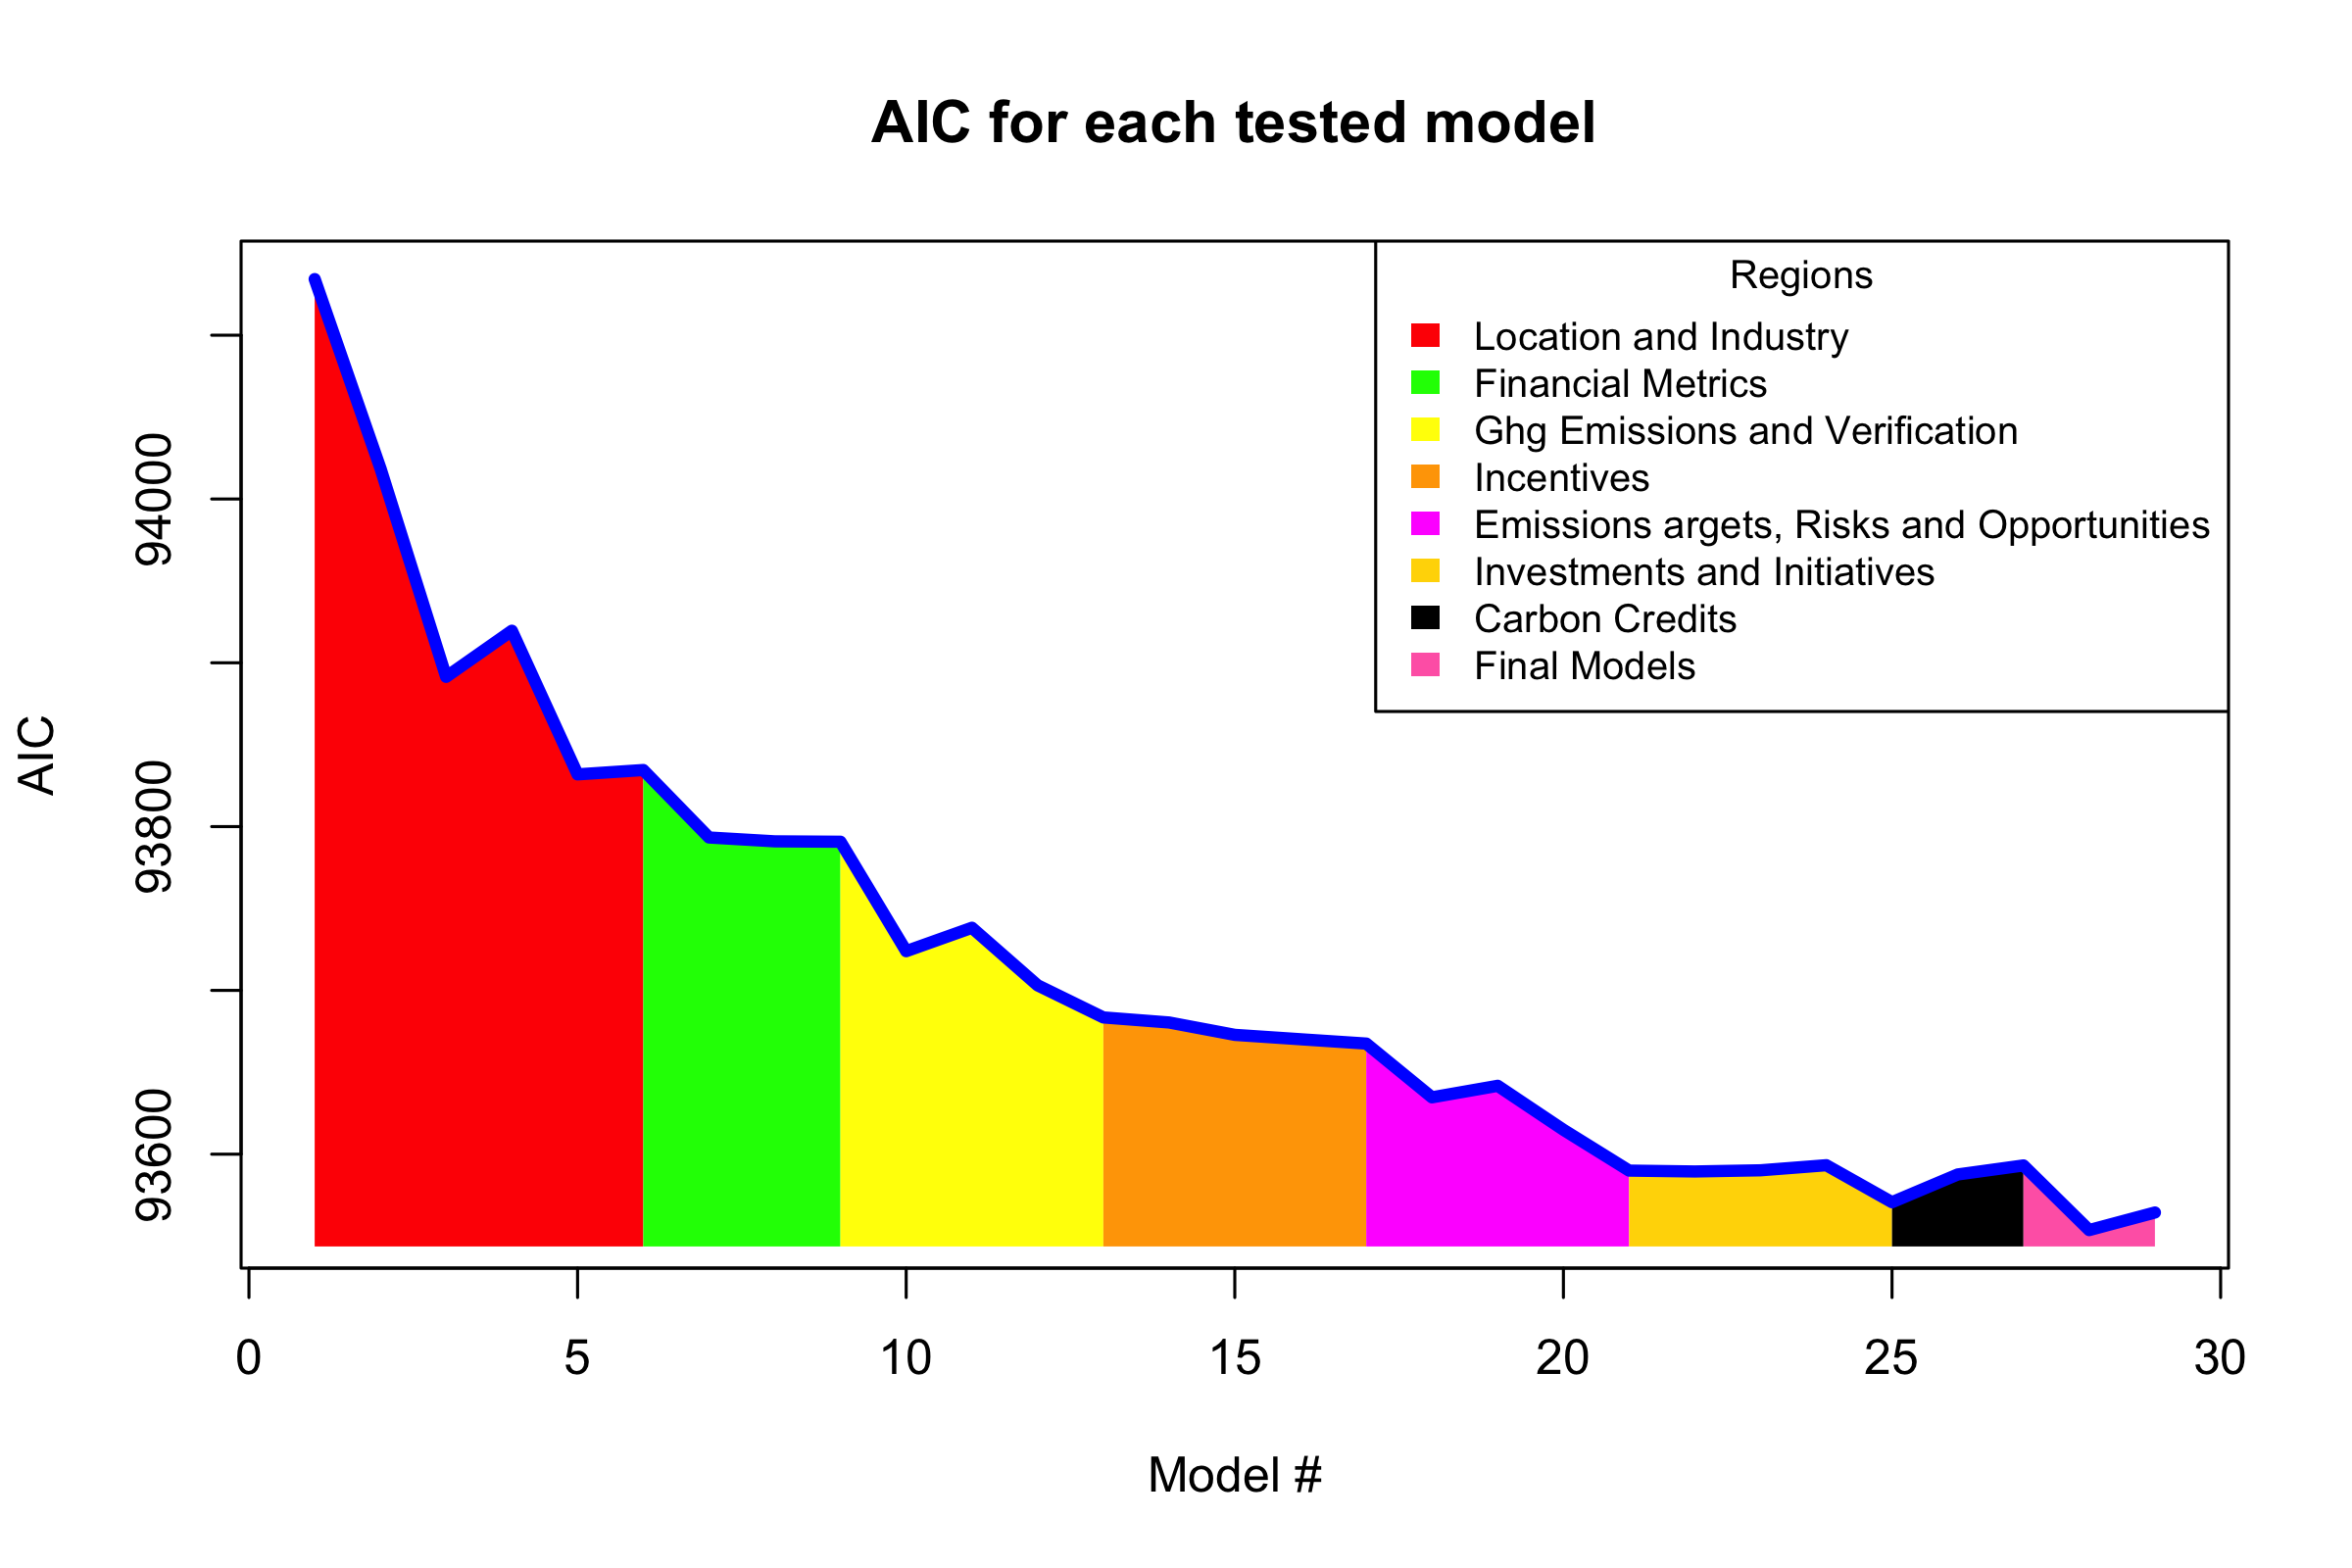
\includegraphics[width=\linewidth]{../notebooks/R/aic.png}
    \caption{AIC of all tested models by model iteration}
    \label{AIC}
\end{figure}

\subsection{Discussion}

\begin{itemize}
    \item We observe how methane emissions is significant at the $1\%$ level when forecasting next year decarboninzation rate, while it is not significan when the response variable is same year decarbonization rate. This is an interesting result and seems to suggest that methane emissions are correlated more with future struggle to decarbonize compared to present decarbonizaion. 
    \item Overall, in model (2) nearly all the predictos are significant, with most being significant at the $1\%$ level. Additionally Figure \ref{AIC} shows how in all model iterations performed in this chapter, we manage to reduce the AIC significantly with the addiiton of significant predictors and the inclusion of relevant random effects. In the final stages, the AIC plateaus, signaling that successive models will only be marginally better than our current final one which strikes a good balance between number of features, interpretability, and forecasting accuracy.
    \item \textbf{Next Steps:} In the following chapter, we will test the prediction accuracy of the final model and use it as a benchmark to develop nonparamatric and more advanced modeling techiques, prioritizing prediction accuracy over interpretability.
\end{itemize}